\chapter{V2V Vehicle Implementation}

\section{Inertia Measurement Unit (IMU)}
\subsection{The data collected and the used sensor}
There are many scenarios for a moving car; starting the engine and going from still to a certain speed, stopping suddenly when the traffic sign becomes red, speeding up when going on highway, … etc. In these scenarios, the common thing is the changing of the speed due to acceleration. So, it was necessary to sense and collect the acceleration information.
To get the acceleration information, an MPU6050  IC is used. It contains a 3-axis gyroscope and a 3-axis accelerometer. So, the data collected from this IC is the acceleration from the 3-axis accelerometer, and the angular speed from the 3-axis gyroscope. The accelerometer is made using MEMS technology. The direction of the acceleration and angular speed for every axis is shown in figure \ref{fig:orientation} .
\begin{figure}[h]
    \centering
    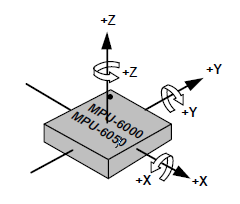
\includegraphics{figure/5-1.png}
    \caption{Orientation of Axes of Sensitivity and Polarity of Rotation}
    \label{fig:orientation}
\end{figure}
\clearpage
To use this IC, the module GY-521 MPU6050 is used. The module is shown in figure \ref{fig:mpu6050}.

\begin{figure}[h]
    \centering
    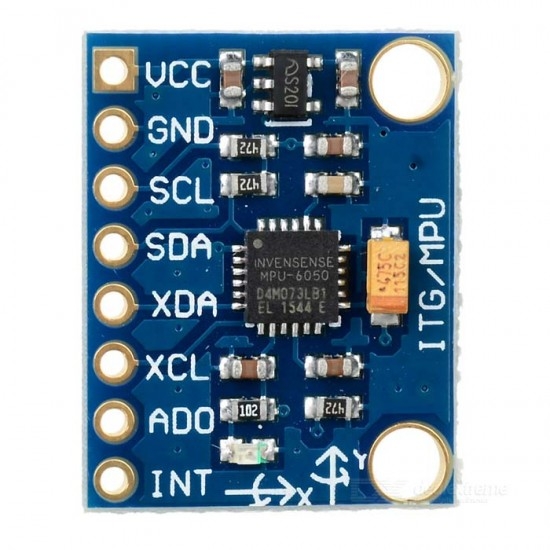
\includegraphics[scale=.5]{figure/5-2.jpeg}
    \caption{GY-521 MPU6050}
    \label{fig:mpu6050}
\end{figure}

The features of this module are as following below:
\begin{itemize}
    \item Power supply: 3-5V.
    \item Communication modes: standard I2C communications protocol.
    \item Chip built-in 16bit AD converter, 16-bit data output.
    \item Tri-Axis angular rate sensor (gyroscope) with a sensitivity up to 131 LSBs/dps and a full-scale range of ±250, ±500, ±1000, and ±2000dps.
    \item Tri-Axis accelerometer with a programmable full-scale range of ±2g, ±4g, ±8g and ±16g.
\end{itemize}

Although this module has both accelerometer and gyroscope, but the focus would be on the acceleration and not the angular speed.
Theoretically, the orientation of the car and its heading can be calculated from the angular speed by integrating the angular speed of the Z-axis as the equation below.
\[ \omega = \frac{d \theta}{dt}\]
\[ \theta = \int_{}^{} \omega \,dx \]

But this is not applicable at hardware level, due to the existence of noise. By adding noise to the system, the equation becomes as following below.
\[ \theta = \int_{}^{} \omega \,dx + \int_{}^{} N \,dt \]
\[ \theta = \theta_{theoretical} + \int_{}^{} N \,dt \]
The noise is integrated with respect to time. So, it  is accumulating with time. That makes the value read from the gyroscope in constant increasing due to noise and not reliable.
To solve this problem, a compass is needed to detect the orientation of the car. This would be discussed later in this chapter.

\subsection{The configuration of the sensor}
\subsubsection{Configuring the I2C address}
As discussed earlier, the GY-521 MPU6050 module uses the I2C communication protocol to communicate with the microcontroller. The I2C communication protocol depends on the addresses of the master and the slave to be able to communicate with each other. So, the address of this module should be known to the microcontroller to be able to communicate with it.
This module can have two different addresses, this is helpful if it was needed to work with two of these modules. So, every module has a different address, and the microcontroller can communicate with each one separately. The address of the module is set using the pin AD0. The next table shows the address of this module in different states of the pin AD0.
\begin{table}[h]
\def\arraystretch{1.5}
\centering
\begin{tabular}{| c | c |}
\hline
 \textbf{AD0 State} &  \textbf{I2C Address} \\
 \hline
 Low &  $(1101000)_2$ \\
 \hline
 High & $(1101001)_2$ \\
 \hline
\end{tabular}
\end{table}

The user chooses the address by hardware, using the AD0 pin, and configure it in the code.
\clearpage
\subsubsection{Configuring the accelerometer scale}
This module also has a programmable full-scale range. It can be four different ranges as discussed earlier. But there is trade off between the range and the resolution of the accelerometer. As the range increases, the resolution increases. The next table shows the relation between the scale and the resolution of this module. The gravity is assumed to be 10 m/s2.

\begin{table}[h]
\def\arraystretch{1.5}
\centering
\begin{tabular}{| c | c |}
\hline
 \textbf{Scale (m/$s^2$)} &  \textbf{Resolution (m/$s^2$)} \\
 \hline
 -20 : +20 &  $610 * 10 ^ -6$ \\
 \hline
 -40 : +40 & $1.22 * 10 ^ -3$ \\
 \hline
  -80 : +80 & $2.44 * 10 ^ -3$ \\
 \hline
  -160 : +160 & $4.88 * 10 ^ -3$ \\
 \hline
 
\end{tabular}
\end{table}
The user configure the range in the code.
\subsubsection{Configuring the order of the LPF}
This module has an internal digital low pass filter (DLPF) to reduce the noise. The user can configure the order of this filter. The higher the order of the DLPF, the smaller the bandwidth, thus the lower the noise effect. But there is tradeoff between the bandwidth of the DLPF and the delay. The higher the order of DLPF, the higher the delay. The next table shows the relation between the delay and the order of the DLPF.

\begin{table}[h]
\def\arraystretch{1.5}
\centering
\begin{tabular}{| c | c | c |}
\hline
 \textbf{DLPF Order} &  \textbf{Bandwidth (Hz)
}  & \textbf{Delay (ms)}\\
 \hline
 0 &  260 & 0 \\
 \hline
1 &  184 & 2.0 \\
 \hline
 2 &  94 & 3.0 \\
 \hline
3 &  44 & 4.9 \\
 \hline
4 &  21 & 8.5 \\
 \hline
 5 &  10 & 13.8 \\
 \hline
 6 &  5 & 19.0 \\
 \hline

\end{tabular}
\end{table}

The user configures the order of DLPF in the code.
\clearpage
\subsubsection{Configuring the sample rate}
The sample rate of this module is following the next formula

\[sample \! rate = \frac{Gyroscope Output Rate}{Prescaler + 1} \]
The gyroscope output rate is 8 kHz when the DLPF is disabled and 1 kHz otherwise.
The user can configure the sample rate using the prescaler value. The prescaler is an unsigned 8-bit number, so it varies from 0 to 255.
The user configures the sample rate in the code.

All the previous configurations that the user could change in the code is done in the file “imu\_config.h” where the configuration is done easily as shown in the code below.

\begin{lstlisting}

#ifndef	__IMU_CONFIG_H__
#define	__IMU_CONFIG_H__
/*	Defining the state of the pin AD0 of the IMU. */
#define	IMU_AD0_STATE					IMU_AD0_SET
/*	Defining the scale of the gyroscope. */
#define IMU_GYRO_SCALE					IMU_GYRO_SCALE_1000
/*	Defining the scale of the accelerometer. */
#define IMU_ACCEL_SCALE					IMU_ACCEL_SCALE_4G
/*	Defining the digital low pass filter(DLPF) order. */
#define	IMU_DLPF_ORDER					0x05UL
/*	Defining the state of the pin AD0 of the IMU. */
#define	IMU_SAMPLE_RATE_PRESCALER		0x00UL
#endif

\end{lstlisting}

\subsection{The functions of this sensor driver}
There are three main functions to be used by the user.
\begin{enumerate}
    \item \textbf{void HAL\_IMU\_Init(I2C\_HandleTypeDef *I2Cx)
    \item \textbf{void} HAL\_IMU\_Read\_Accel(I2C\_HandleTypeDef *I2Cx, IMU\_TypeDef *DataStruct)}
    \item \textbf{HAL\_StatusTypeDef HAL\_IMU\_Test(I2C\_HandleTypeDef *I2Cx)}
\end{enumerate}
\clearpage
These functions are used in the main as the user wants to its application.
\begin{enumerate}
    \item \textbf{void HAL\_IMU\_Init(I2C\_HandleTypeDef *I2Cx)}
    \begin{figure}[h]
        \centering
        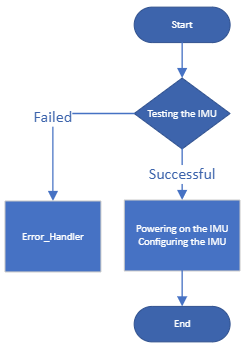
\includegraphics{figure/5-3.png}
        \caption{Flow chart of the initiation function}
    \end{figure}
    \begin{itemize}
    \item This function takes the I2C peripheral used to communicate with the IMU as input.
    \item This function does not return.
    \item It starts by testing the IMU using the function \textbf{HAL\_IMU\_TEST} which would be discussed later.
    \item If the test went successful, the program continues. But if it failed, the program calls the function \textbf{Error\_Handler} which is configurable by the user.
    \item The IMU is powered on and configured, as the user choose in “imu\_config.h” file, by writing specific values into its registers.
    \end{itemize}
    \item \textbf{void HAL\_IMU\_Read\_Accel(I2C\_HandleTypeDef *I2Cx, IMU\_TypeDef *DataStruct)}
    \begin{figure}[h]
    \centering
    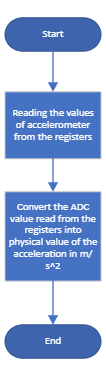
\includegraphics{figure/5-4.png}
    \caption{Flow chart of the reading function}
\end{figure}
    \begin{itemize}
        \item This function takes the I2C peripheral used to communicate with the IMU and pointer to the data struct containing the variables to store the accelerations as inputs.
        \item This function does not return.
        \item It starts by reading the values of the accelerations for the three axes in the registers of the MPU6050.
        \item These values are signed 16-bit value representing the acceleration of the car in the three axes.
        \item These values are then converted into a number representing the acceleration in $m/s^2$ and saved in the corresponding variables in the data struct.
        \item These conversions depend on the scale configured for the MPU6050.
        \item The conversion is done using the following formula
        \[ a = (16 - bit value) * (Resolution)\]
    \end{itemize}
    \item \textbf{HAL\_StatusTypeDef HAL\_IMU\_Test(I2C\_HandleTypeDef *I2Cx)}
    
    
    \begin{itemize}
        \item This function takes the I2C peripheral used to communicate with the IMU as input.
        \item This function returns the status of the test.
        \item There is a register in the module called WHO\_AM\_I register, this register is read only register with a fixed value equal to 0x68 in hexadecimal format.
        \item The test reads the value of this register and compare it to the value 0x68. If it is equal to this value, then the test is successful and it returns HAL\_OK. But if it was something else, the MPU6050 is reset by software and  it tries again to read the register for a certain number of tries.
        \item If the number of tries have exceeded the allowed number of tries, the function returns HAL\_ERROR.
    \end{itemize}
    \begin{figure}[h]
    \centering
    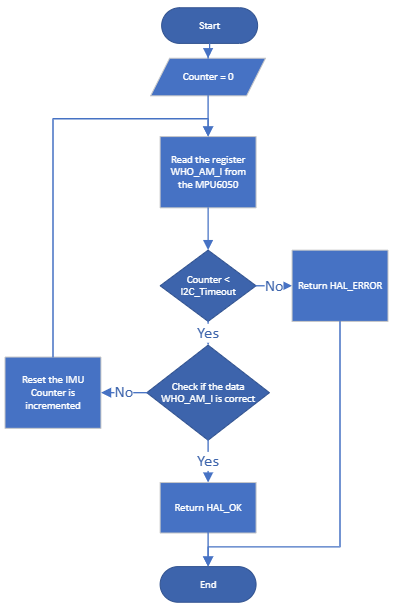
\includegraphics{figure/5-5.png}
    \caption{Flow chart of the testing function}
    \end{figure}
\end{enumerate}
\clearpage
\subsection{Testing the sensor}
To evaluate the sensor and its output values, the gravity is used.
We position the module in three different positions and read the values of acceleration from the three different axes.
\textit{The next table shows the three different positions.}


\begin{figure}[h]
    \centering
    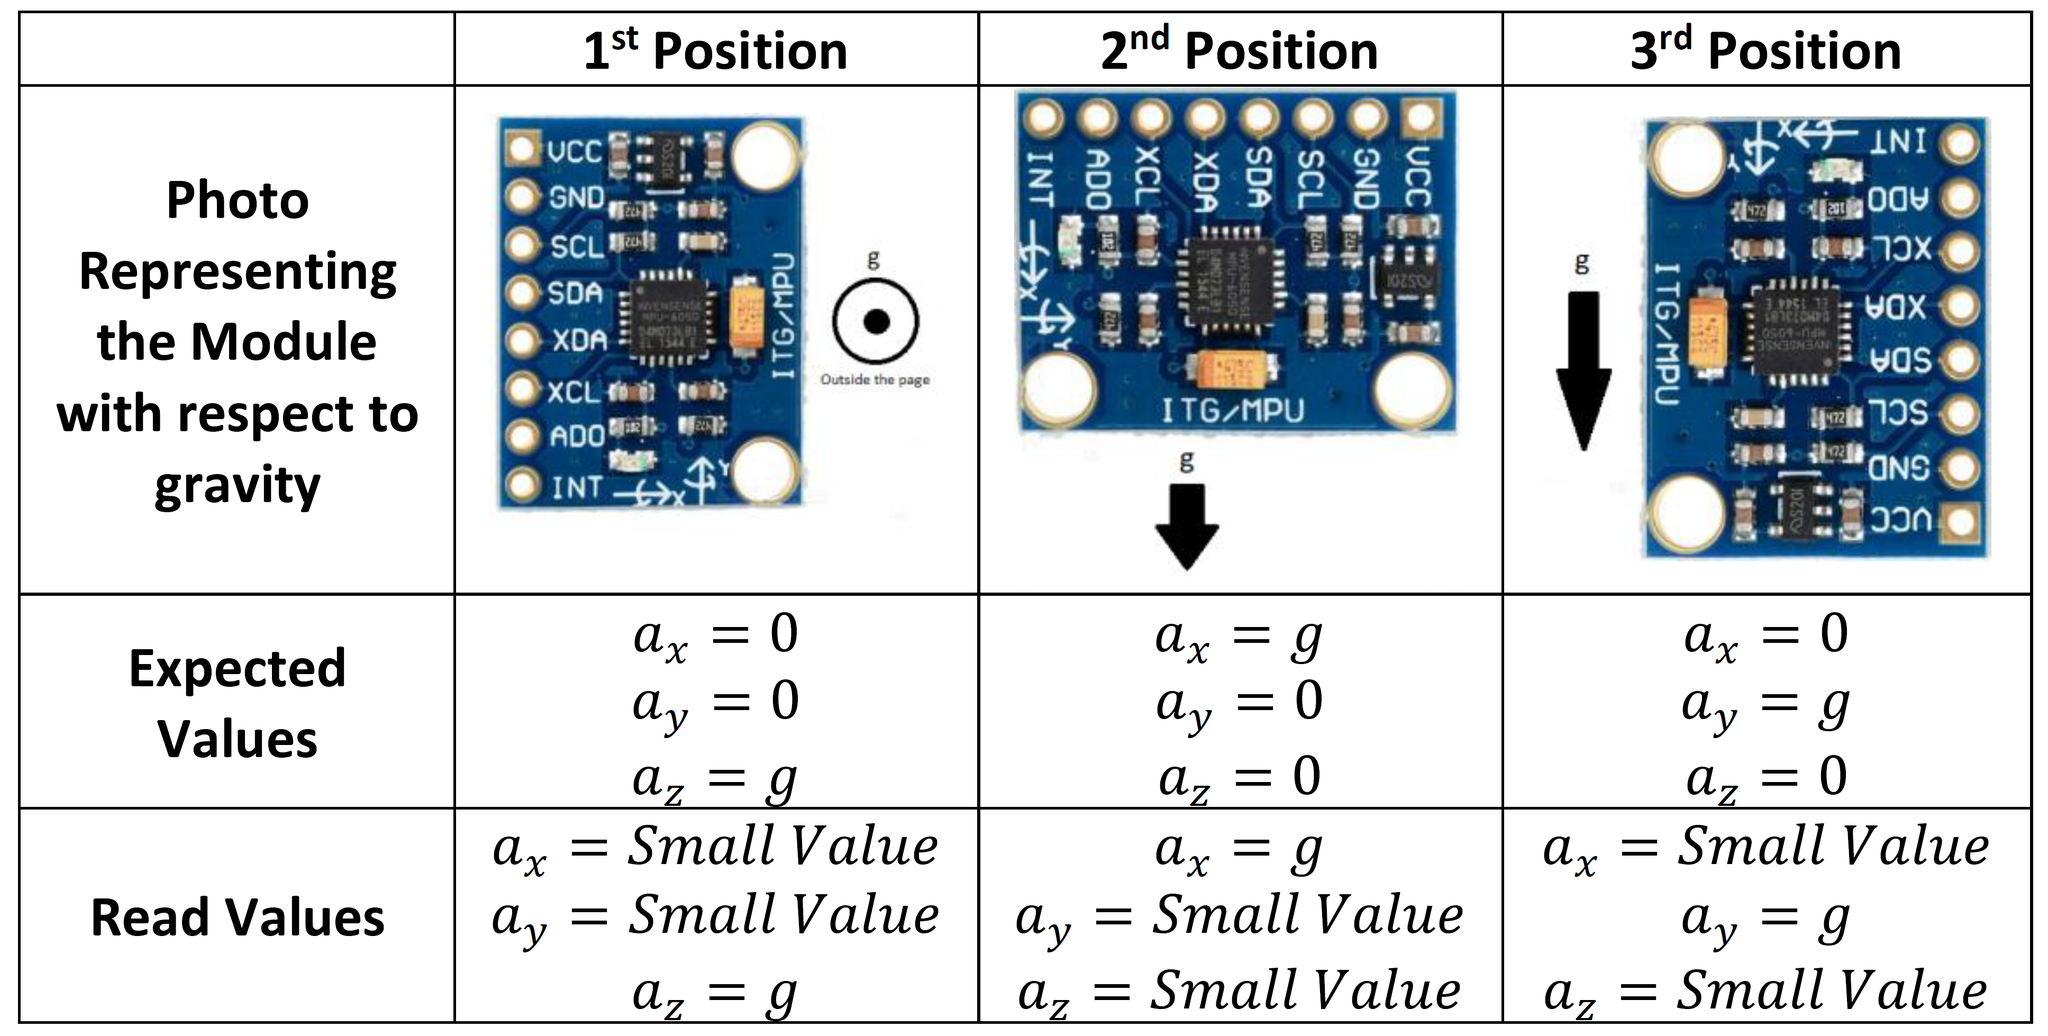
\includegraphics[scale=.2]{figure/5-6.png}
    \caption{IMU in three different positions}
\end{figure}
This means that the test went successful, and the IMU is working fine.

\section{Speed Measurement Unit}

\subsection{The data collected and the used sensor}
The main variable to be monitored in modern cars as well as ancient cars is the speed. Any car must have a speed monitoring system in it whether it is an analog system such as a pointer on scale or a digital system such as a lcd displaying the speed. This shows how important is the speed information for the vehicle.
There were two options for selecting the sensor used for the sensing the speed information.
\begin{figure}[h]
    \centering
    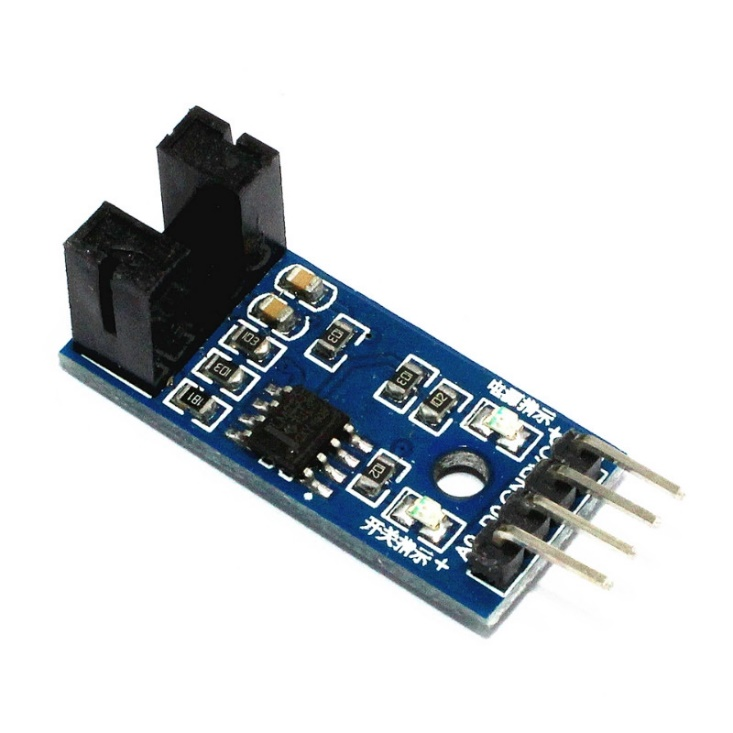
\includegraphics[scale=.5]{figuresEncoder/1.jpeg}
    \caption{IR Encoder}
\end{figure}
\begin{figure}[h]
    \centering
    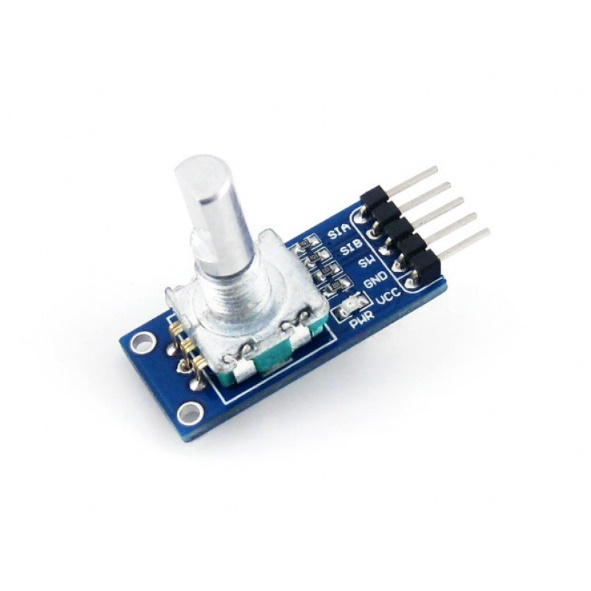
\includegraphics{figuresEncoder/2.jpeg}
    \caption{Shaft Rotary Encoder}
\end{figure}

The first option was the shaft rotary encoder. 
The working principle of this sensor is that there are two metal contacts separated apart from each other, and the common pin is a gear. So, when the tooth of the gear touches the metal it the output is high, otherwise the output is low. So, when the shaft moves, a square pulse is generated on the two outputs, and since the two metals are separated apart, the two square waves are phase shifted.

\begin{figure}[h]
    \centering
    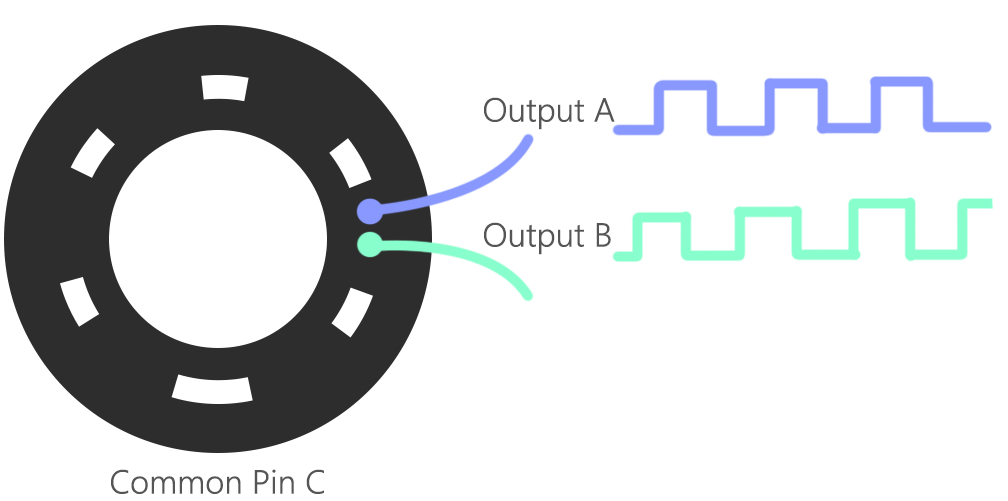
\includegraphics[scale=.4]{figuresEncoder/3.png}
    \caption{The working principle of shaft rotary encoder}
\end{figure}

 The advantages of the shaft rotary encoder
\begin{enumerate}
    \item Its simple system.
    \item It can detect the direction of the rotation whether it is clockwise (CW) or counterclockwise (CCW). This is done using the phase shift information between the two square pulses.
    \item It is compatible with the micro controller using the encoder mode in the timer peripheral.
\end{enumerate}

The disadvantages of the shaft rotary encoder
\begin{enumerate}
    \item There is bouncing because the system is mechanical switch. This problem can be solved using digital low pass filter (DLPF) in the timer peripheral in the encoder mode.
    
    \item It is connected directly to the motor which is seen as a load and can effect the speed of the motor specially if the shaft of the sensor is stuck.
    
\end{enumerate}
The second option was the infra-red (IR) encoder .
The working principle of this sensor is that there is an IR LED is a side, an IR detector in the other side, and a comparator. When the beam is continuous from the LED to the receiver, the output from the module is high. When the beam is blocked and was not received by the IR detector, the output from the module is low.

\begin{figure}[h]
    \centering
    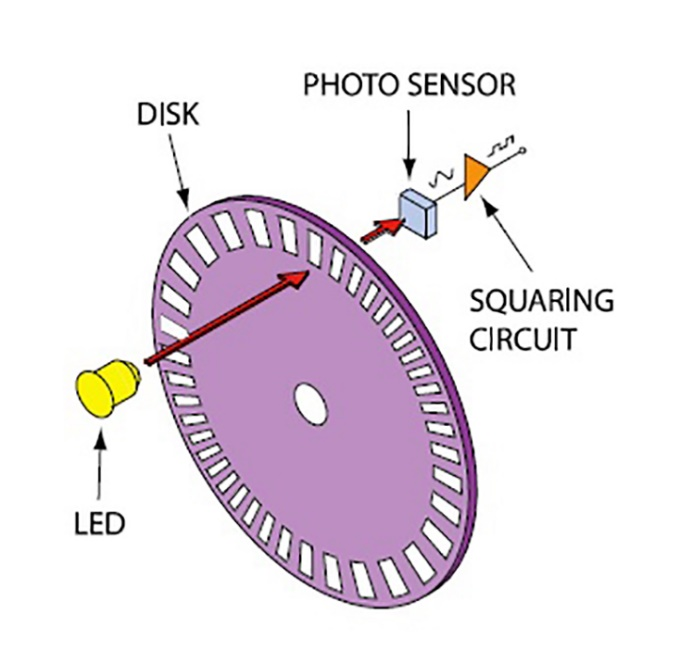
\includegraphics[scale=.7]{figuresEncoder/4.jpeg}
    \caption{The working principle of the IR encoder}
\end{figure}

The advantages of the IR encoder
\begin{itemize}
    \item There is no physical contact between the sensor and the motor. So, there is no load on the motor.
    \item It is very fast and reliable.
    \item The square wave output is perfect and has no bouncing.
\end{itemize}

The disadvantages of the IR encoder
\begin{itemize}
    \item It can’t detect the direction of the rotation.
\end{itemize}
The sensor used in this project would be the IR encoder.

\subsection{The configuration of the sensor}
The  sensor is used to calculate the revolution per minute (RPM).
The calculation of the RPM is following the next formula
\[ RPM = \frac{No. of revolutions}{Time elapsed}\]

There are two timer peripherals used to calculate the RPM; one is used to act as counter to count the number of revolutions, the other is used to act as timer to act as stopwatch for the time elapsed.
To calculate the RPM in this project, the number of revolutions is sampled after a specific period the user configure it previously.

\clearpage
\subsubsection{Configuring the number of pulses in one revolution}

There is a wheel with slots in it is attached to the motor shaft and displaced between the IR LED and IR receiver, the number of slots in the wheel represents the number of pulses in one cycle.
\begin{figure}[h]
    \centering
    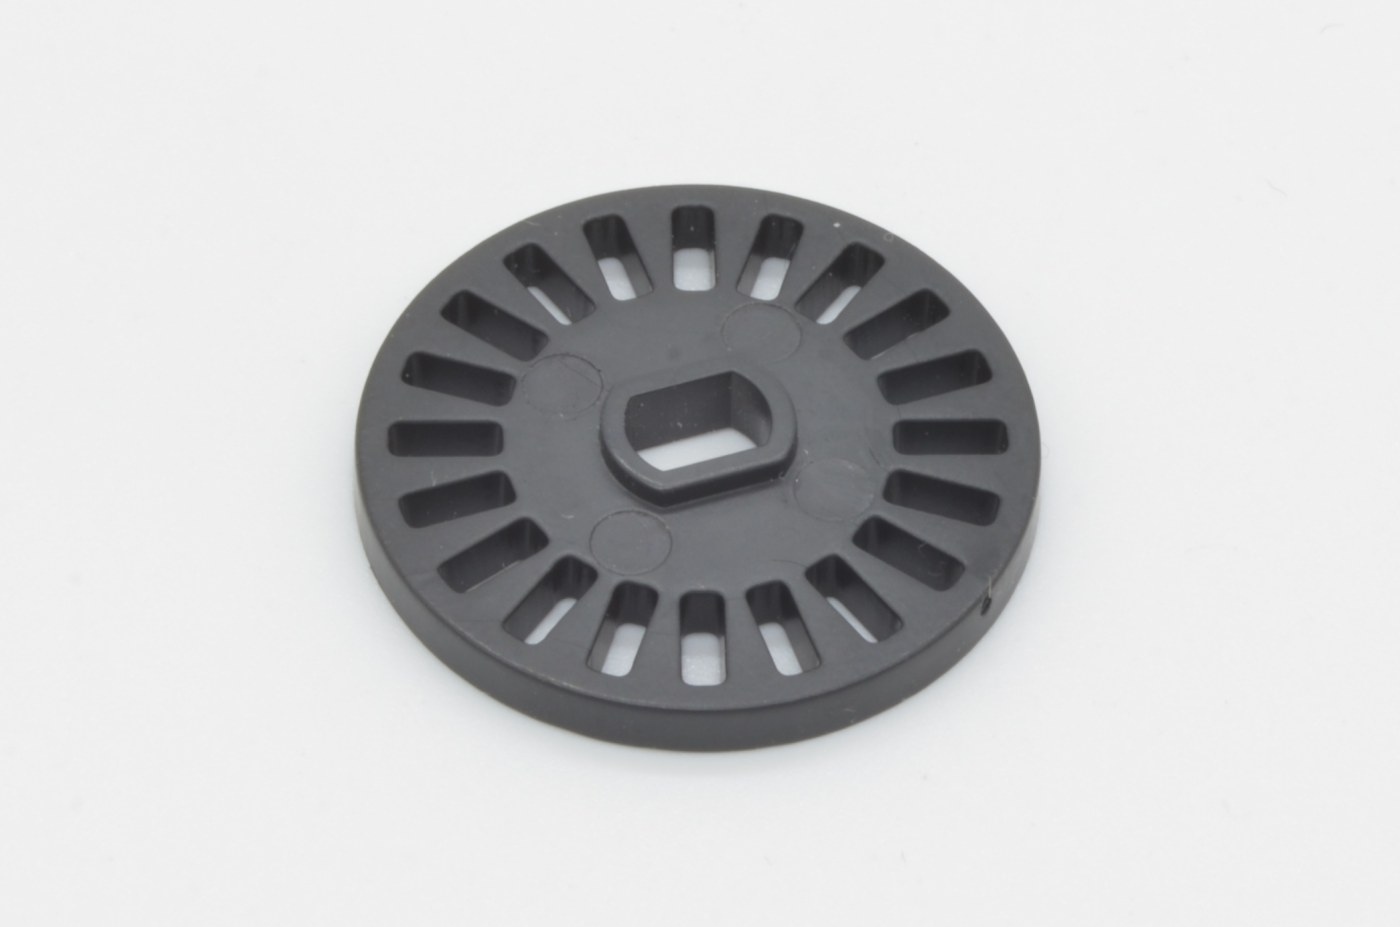
\includegraphics[scale=.2]{figuresEncoder/5.jpeg}
    \caption{The wheel connected to the shaft of the motor}
\end{figure}
The user configures this number in the code. In this project it is 20 slots.

\subsubsection{Configuring the counter}
To configure the counter, the clock source of the timer is chosen to be ETR2. This allows the timer peripheral to update with external clock.
Note that only timer 1 and timer 2 can be counter from the external source.
Also, the auto reload value must be enabled.
\begin{figure}[h]
    \centering
    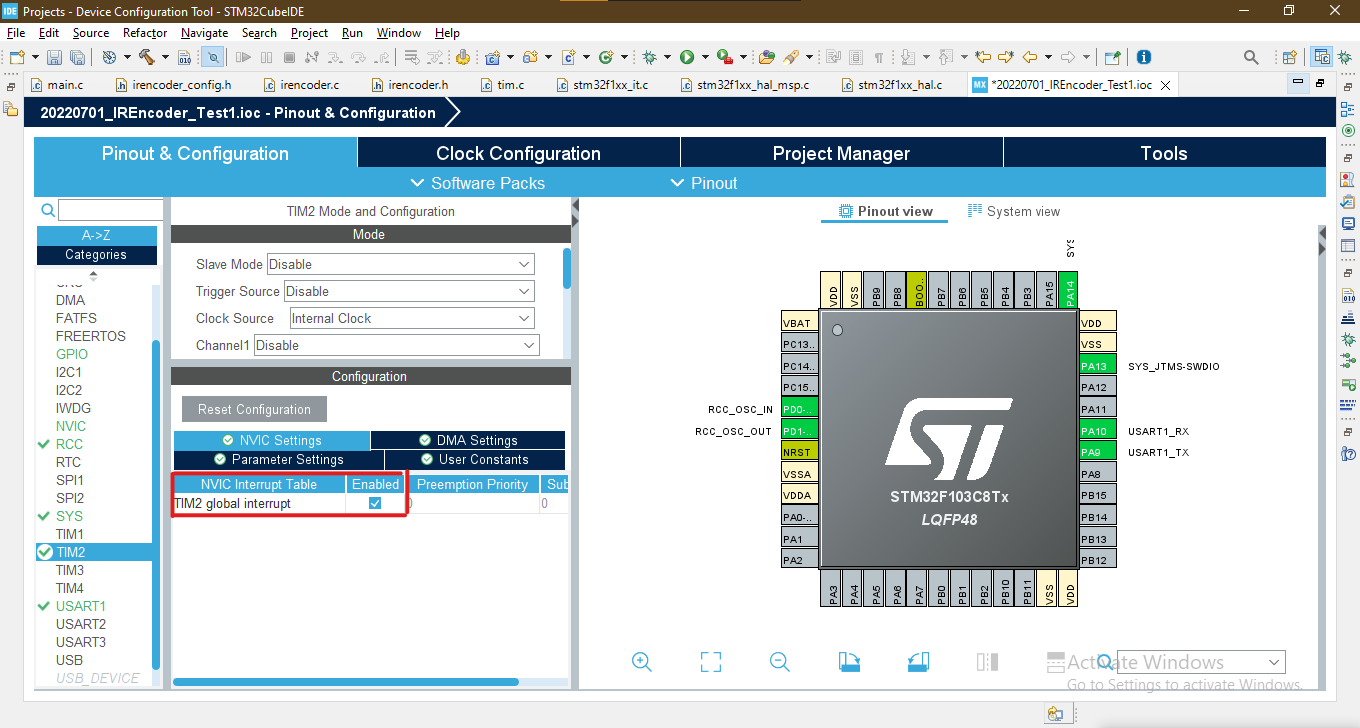
\includegraphics[scale=.4]{figuresEncoder/6.png}
    \caption{Configuring the counter in STM32CubeIDE}
\end{figure}
The user configures this in the STM32CubeIDE program.
\clearpage
\subsubsection{Configuring the timer}
To configure the timer, the clock source of the timer is chosen to be internal. This allows the timer peripheral to act as clock.
There are two internal clocks for the timers, as shown in the block diagram, from the datasheet, that timer 1 clock source is APB2, and the other timers are from APB1.

\begin{figure}[h]
    \centering
    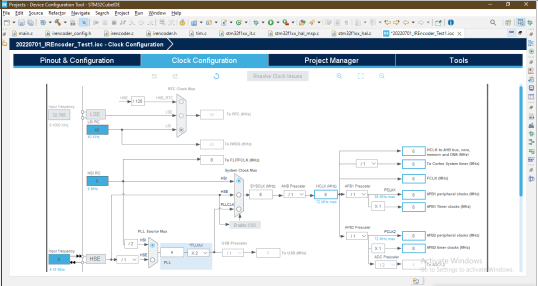
\includegraphics[scale=.8]{figuresEncoder/7.png}
    \caption{Clock Configuration in the STM32CudeIDE}
\end{figure}

\begin{itemize}
    \item The auto reload value must be enabled.
    \item The interrupt of this timer must be enabled.
\end{itemize}

\begin{figure}[h]
    \centering
    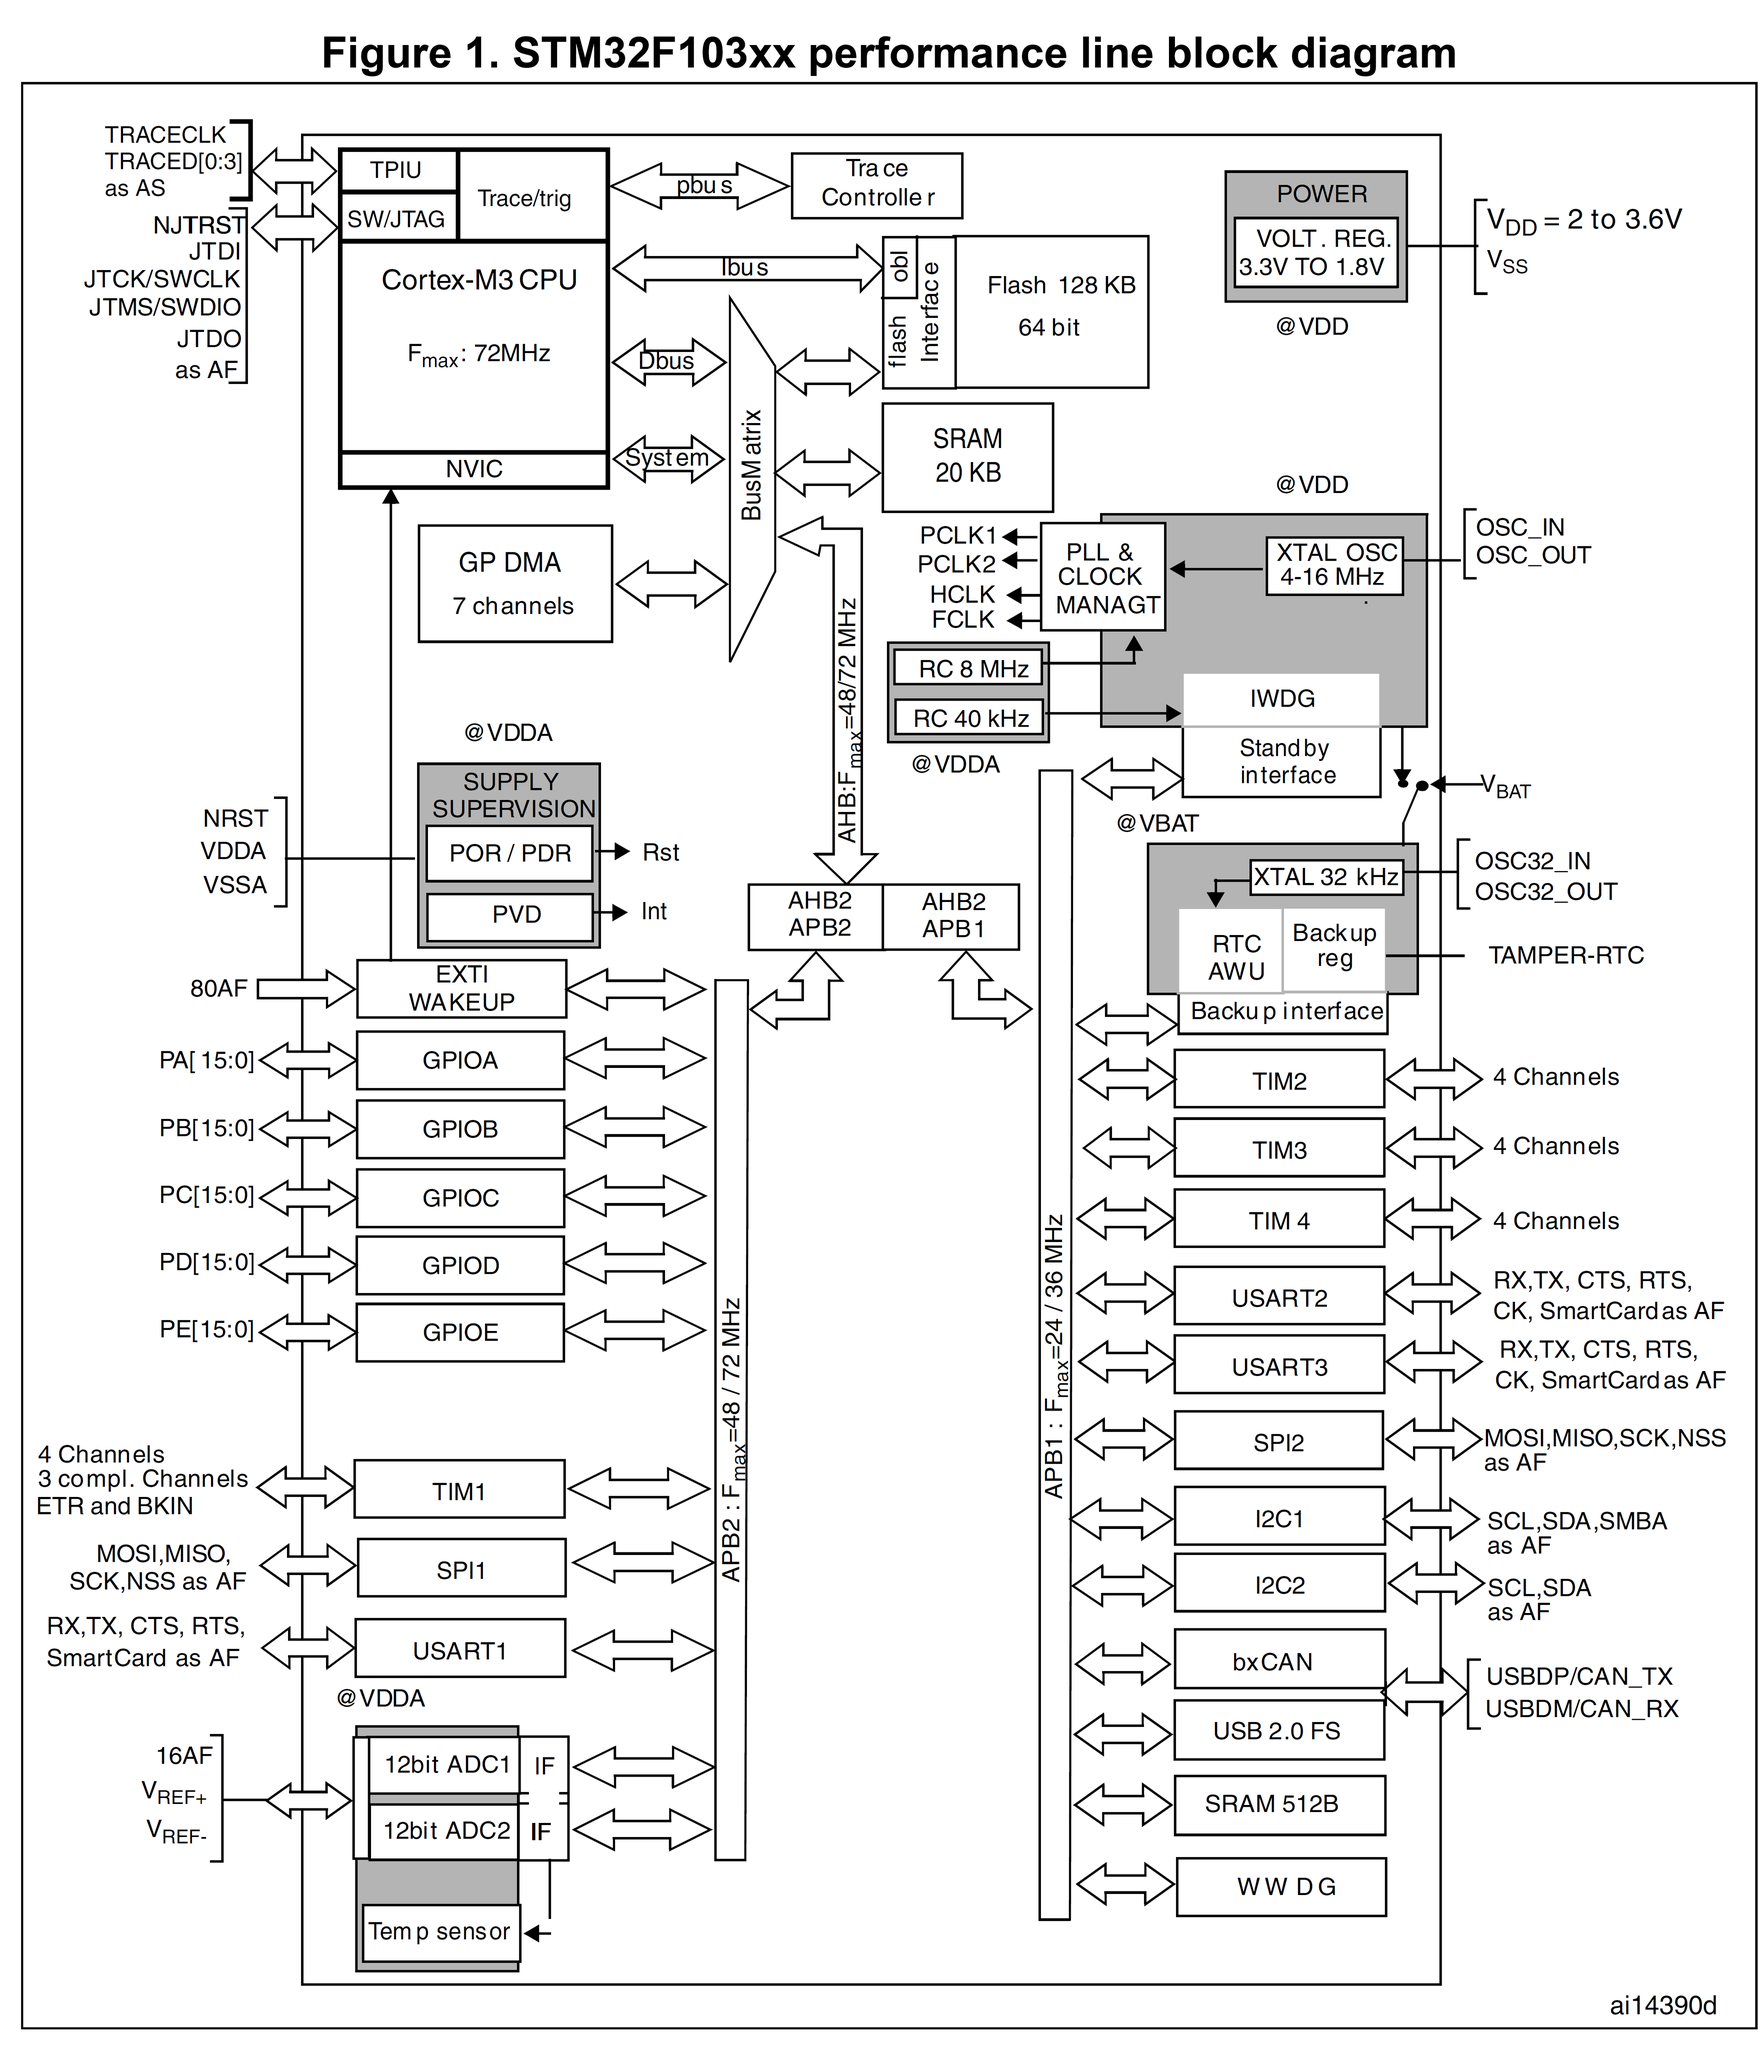
\includegraphics[scale=.22]{figuresEncoder/8.png}
    \caption{STM32F103C8T6 Block Diagram}
\end{figure}

\begin{figure}[h]
    \centering
    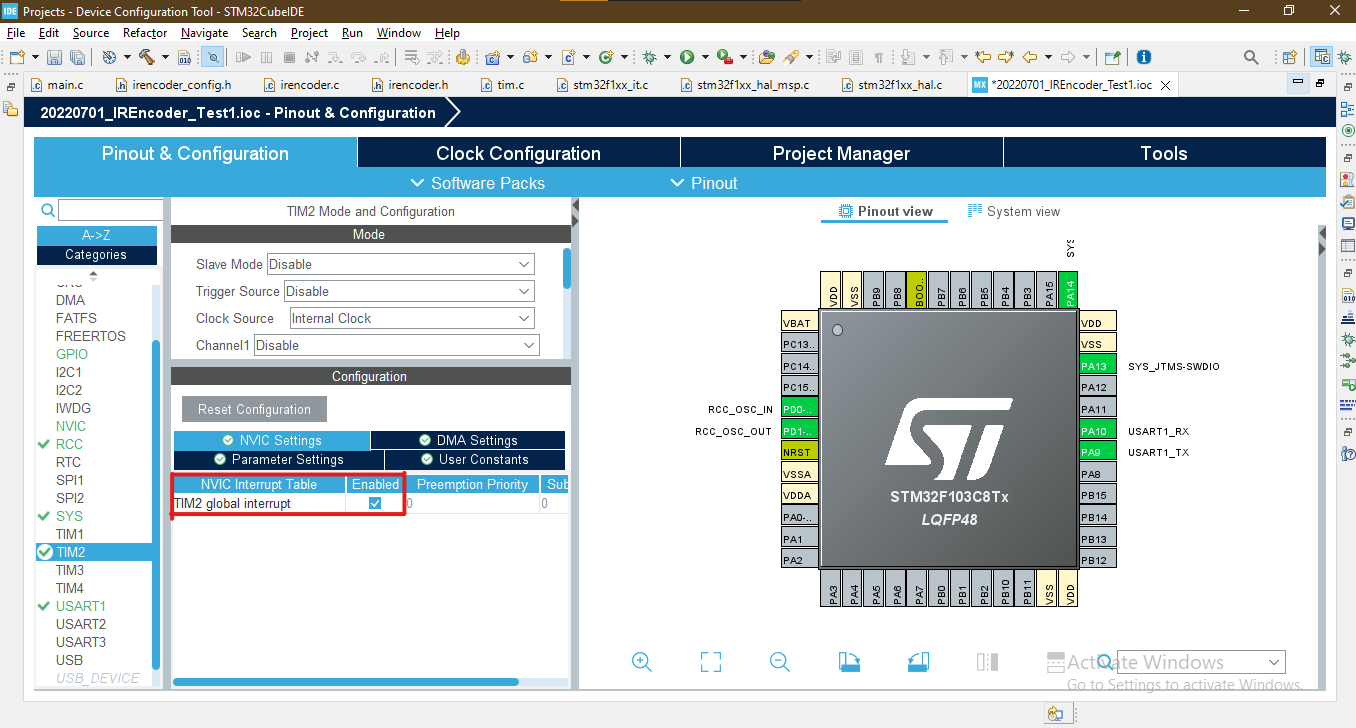
\includegraphics[scale=.34]{figuresEncoder/9.png}
    \caption{Configuring the timer in STM32CubeIDE (1)}
\end{figure}

\begin{figure}[h]
    \centering
    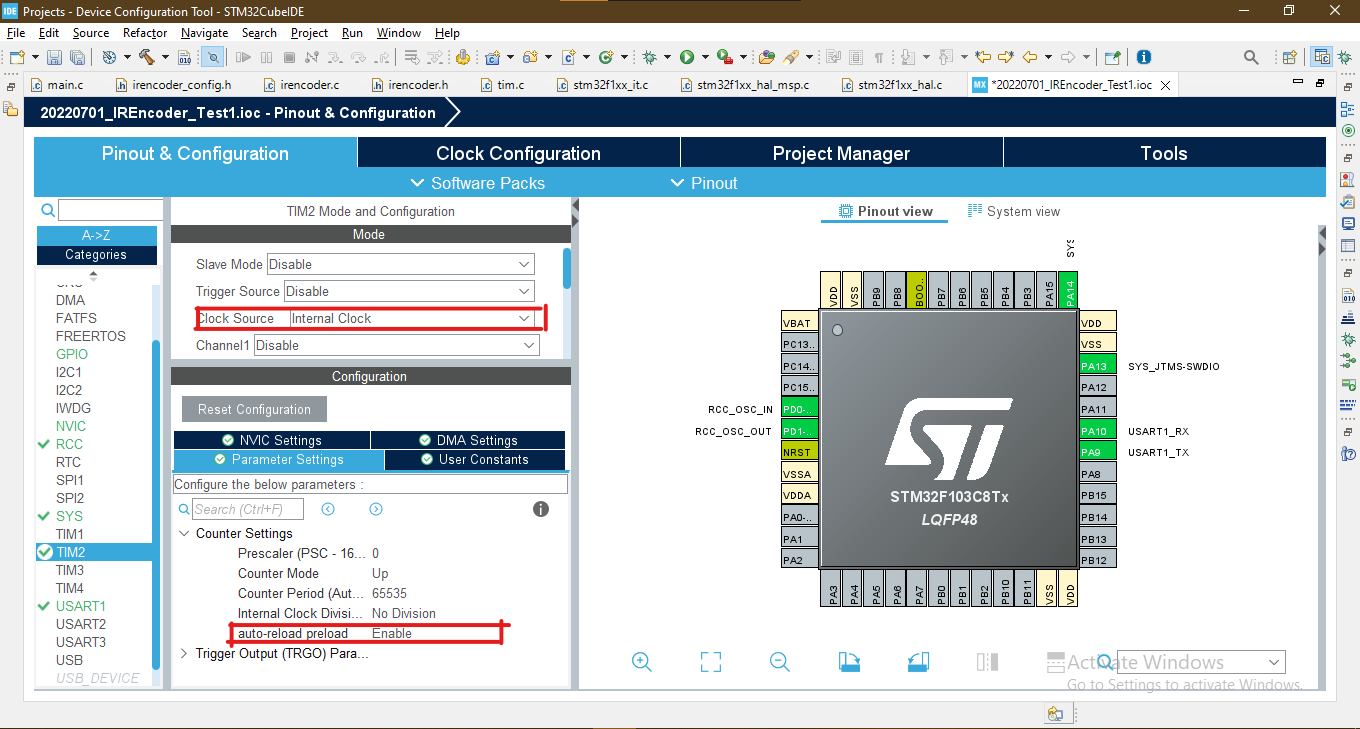
\includegraphics[scale=.33]{figuresEncoder/10.png}
    \caption{Configuring the timer in STM32CubeIDE (2)}
\end{figure}
\clearpage
\subsubsection{Configuring the timer clock}
Configuring the timer clock is done by the page of clock configuration in the STM32CudeIDE program as discussed earlier. But the additional thing to do is to configure the value of this clock in the code to help the program to calculate the RPM correctly. This configuration is done in the code.

\subsubsection{Configuring the period}
As discussed earlier, to calculate the RPM, the number of revolutions is sampled after a fixed period. This period is configured by the user.
This configuration is done in the code.
All the configurations that were done in the code, are modified in the file “irencoder\_config.h” easily.

\begin{lstlisting}
#ifndef __IRENCODER_CONFIG_H__
#define __IRENCODER_CONFIG_H__
/*	Defining the number of slots of the wheel attached to the motor. */
#define IRENCODER_ONE_CYCLE_PULSES		20
/*	Defining the clock frequency of the timer in kHz. */
#define IRENCODER_TIMER_CLK		8000
/*	Defining the method used to calculate the RPM. */
#define IRENCODER_RPM_CALCULATION		IRENCODER_RPM_FIXED_TIME
#endif

\end{lstlisting}

\section{The functions of this sensor driver}
\begin{enumerate}
    \item \textbf{void HAL\_IREncoder\_Start(TIM\_HandleTypeDef *Counter,\\TIM\_HandleTypeDef *Timer)}
    \item \textbf{void HAL\_IREncoder\_Stop(TIM\_HandleTypeDef *Counter, \\TIM\_HandleTypeDef *Timer)}
    \item \textbf{void HAL\_TIM\_PeriodElapsedCallback(TIM\_HandleTypeDef *htim)}
\end{enumerate}
These functions are used in the main depending on the user needs.
\clearpage
\begin{enumerate}
    \item \textbf{void HAL\_IREncoder\_Start(TIM\_HandleTypeDef *Counter,\\TIM\_HandleTypeDef *Timer)}
    \begin{figure}[h]
        \centering
        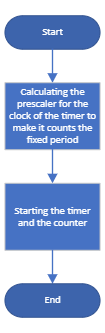
\includegraphics[scale=.6]{figuresEncoder/11.png}
        \caption{Flow Chart of the starting function}
    \end{figure}
    \begin{itemize}
        \item This function takes the timer and the counter as inputs.
        \item This function has no return.
        \item It first configures the timer so that it overflows after the fixed period defined by the user. That is the reason why the timer interrupt is activated. The calculation of the RPM is in the callback function of the timer interrupt.
        \item Starting both the timer and the counter. Notice that the timer is started in interrupt mode and the counter is started in the normal mode.
    \end{itemize}
    
     \item \textbf{void HAL\_IREncoder\_Stop(TIM\_HandleTypeDef *Counter, \\TIM\_HandleTypeDef *Timer)}
    \begin{itemize}
        \item This function takes the timer and the counter as inputs.
        \item This function has no return.
        \item This function has no return.
        \item It stops both the timer and the counter.
    \end{itemize}
    \clearpage
    \item \textbf{void HAL\_TIM\_PeriodElapsedCallback(TIM\_HandleTypeDef *htim)}
    \begin{figure}[h]
        \centering
        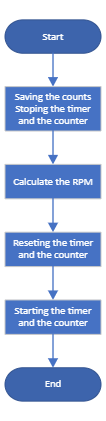
\includegraphics[scale=.6]{figuresEncoder/12.png}
        \caption{Flow Chart of the callback function}
    \end{figure}
    \begin{itemize}
        \item This function isn’t called by the user, but it starts when an interrupt occurs.
        \item It saves the value stored in the register of the counter as pulses.
        \item It stops the counter and the timer to prevent another interruption during the calculation.
        \item It calculates the RPM as the formula discussed earlier.
        \item It Resets the timer and the counter to be ready for the next iteration and parsing.
        \item The counter and the timer are started.
    \end{itemize}
    
\end{enumerate}
\subsection{Testing the sensor}
To test the sensor, a motor with a relatively known low speed is connected to the IR Encoder, and the RPM value is monitored.
For the test to be successful, the value of RPM from the code calculation should match the value of the RPM from the motor.

\section{Orientation Measurement Unit}
\subsection{The data collected and the used sensor}
The person in the driver seat uses the steering wheel to direct the vehicle into the direction he wants to go. When he wants to go from a lane to another, a signal light is used to inform the other cars in the lane of the sudden change. This shows how important is the heading and the orientation information of the car.
Although there is a gyroscope in this project, but it is discussed in the inertia measurement unit section the reasons why it cannot be used to get the orientation.
So, the sensor used for the orientation and heading information is HMC5883L IC.
This sensor has a 3-axis Magneto resistive which figure \ref{fig:hm5883l} shows the direction of the axes.

\begin{figure}[h]
    \centering
    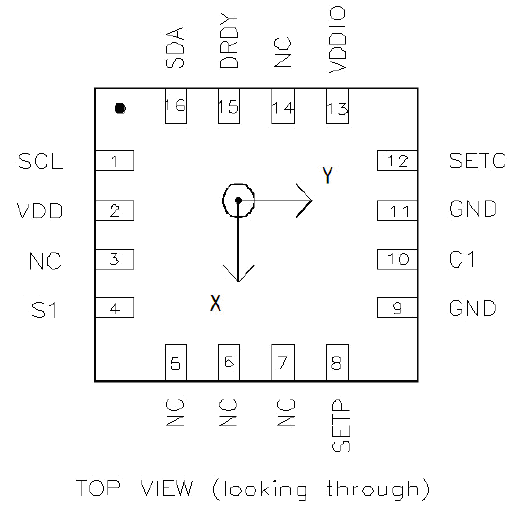
\includegraphics[scale=.6]{figures/1.png}
    \caption{The HMC5883L IC}
    \label{fig:hm5883l}
\end{figure}
\clearpage
The module used is GY-273 HMC5883L.
\begin{figure}[h]
    \centering
    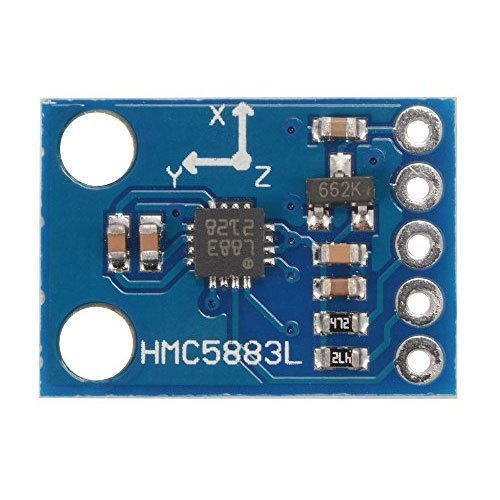
\includegraphics[scale=.5]{figures/2.jpeg}
    \caption{GY-273 HMC5883L Module}
\end{figure}
The main features of this module are as following below.
\begin{itemize}
    \item 3-Axis magneto resistive sensors.
    \item 12-bit analog digital converter.
    \item I2C digital interface.
\end{itemize}

This module is just a magneto sensor. So, it senses the magnetic field of the earth. Where the absolute value of the magnetic field sensed is maxed, it points to either north or south, where the magnetic field is strongest. If this value, the maximum value, is positive , then it points to north. And if this value, the maximum value, is negative, then it points to south.
\clearpage
\begin{figure}[h]
    \centering
    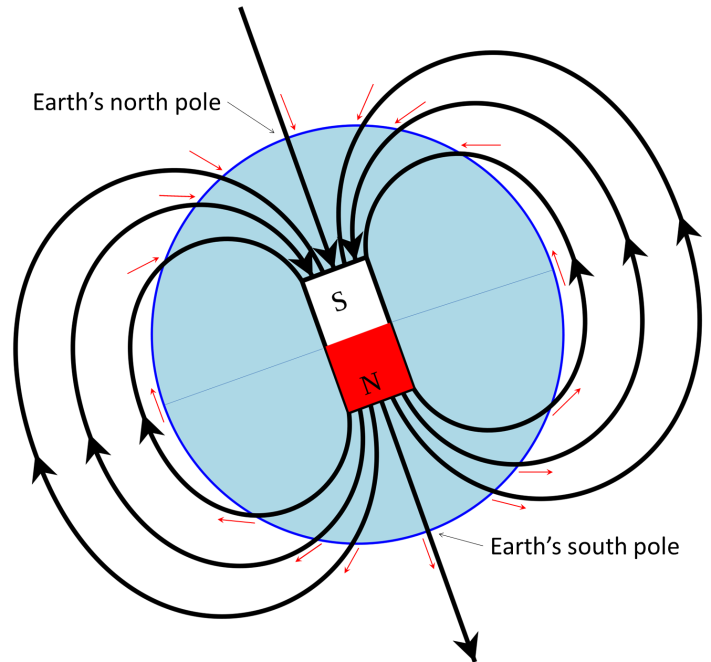
\includegraphics[scale=.3]{figures/3.png}
    \caption{Earth Magnetic Field}
\end{figure}
The working principle of this module is where the magneto sensor senses a positive max value in one of its axes, this axis points to the north. Knowing which direction is the north, the heading and the orientation is known with respect to the north as in maps.
Theoretically, the values sensed from the magneto sensors are moving on a circle its center is the origin point.
Since this module has x-axis and y-axis, this helps to find the directions effectively.
The existing of two axes, x-axis and y-axis, makes determining the angle between the x-axis and the north calculated using the following formula
\[ \theta = tan ^{-1} (\frac{magnetic value \in y-axis}{magnetic value \in x-axis})\]
There is 90 degrees shift between the two axes. So, if y-axis is used to determine the north with respect to itself, all that is needed to done is adding or removing 90 degrees to the output of the previous formula.

\subsection{The configuration of the sensor}
\subsubsection{Calibrating the sensor}
The sensor has a drift in the magneto sensor, that makes the center of the circle is not the origin point.
This can be shown by spinning the module 360 degrees while capturing the values of the magnetic field sensed in the registers of the module.
\clearpage
\begin{figure}[h]
    \centering
    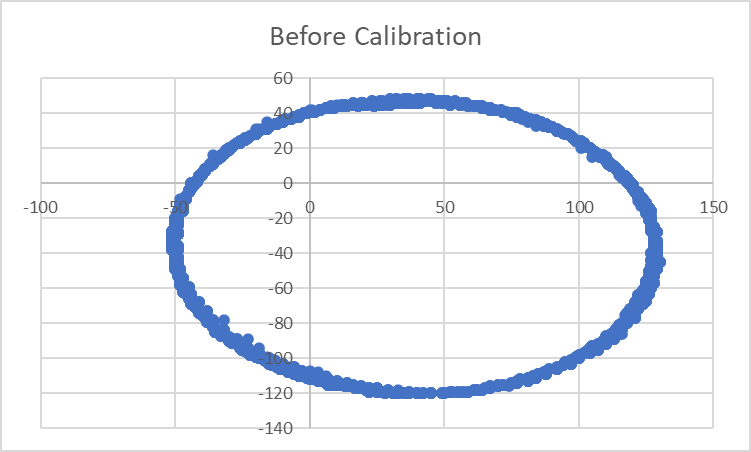
\includegraphics[scale=.3]{figures/4.png}
    \caption{The values of the magnetic fields before calibration}
\end{figure}
These values can be calibrated by calculating the offset of both axes.
The calculation would be following the next formula.

\[x_{new} = x_{dd} - \frac{x_{max} + x_{min}}{2} \]
\[y_{new} = y_{dd} - \frac{y_{max} + y_{min}}{2} \]

\begin{figure}[h]
    \centering
    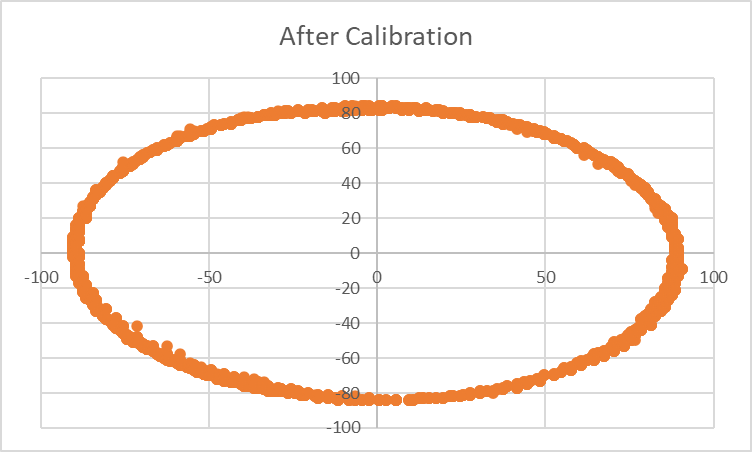
\includegraphics[scale=.3]{figures/5.png}
    \caption{The values of the magnetic fields after calibration}
\end{figure}
These calibrations are done by rotating the module 360 degrees to parse the values and calibrate the offset by code.

\subsubsection{Configuring the average sample rate}
The samples acquired from the magneto sensors can be averaged for more accuracy.
The average sample can be just one sample, two samples, 4 samples, or 8 samples.
The user configures this by the code.
\subsubsection{Configuring the output data rate}
The frequency of reading the value from the magneto sensors and storing into its registers is the data output rate.
The output rate could be one of the following values; 0.75, 1.5, 3, 7.5, 15, 30, or 75 Hz.
The user configures this by the code.
\subsubsection{Configuring the gain}
There are different ranges could be programmed by the user. But there is trade off between the range, or the gain, and the resolution. The higher the range the higher the resolution.
The next table shows the relation between the ranges available in this module and the resolution.

\begin{table}[h]
\def\arraystretch{1.5}
\centering
\begin{tabular}{| c | c |}
\hline
 \textbf{Range (Ga)} &  \textbf{Resolution (mGa/LSB)} \\
 \hline
 -0.88 to +0.88 &  0.73 \\
 \hline
 -1.3 to +1.3 & 0.92 \\
 \hline
 -1.9 to +1.9 & 1.22 \\
 \hline
  -2.5 to +2.5 & 1.52 \\
 \hline
   -4.0 to +4.0 & 2.27 \\
 \hline
   -4.7 to +4.7 & 2.56 \\
 \hline
   -5.6 to +5.6 & 3.03 \\
 \hline
   -8.1 to +8.1 & 4.35 \\
 \hline
 
\end{tabular}
\end{table}
This configuration can be done in the code.
\subsubsection{Configuring the I2C communication protocol}
The I2C can be in standard mode and fast mode.
In standard mode, the clock speed is 100 kHz. In fast mode, the clock speed is 100 kHz.
In fast mode, the clock speed is 400 kHz.
These configurations are done by the code.

All the configurations are modified in the file “compass\_config.h” easily.

\begin{lstlisting}
#ifndef __COMPASS_CONFIG_H__
#define __COMPASS_CONFIG_H__
/*	Defining the samples averaged per measurement output */
#define COMPASS_AVERAGE_SAMPLES		COMPASS_AVERAGE_SAMPLES_1
/*	Defining the data output rate */
#define COMPASS_DATA_OUTPUT_RATE	COMPASS_DATA_OUTPUT_RATE_15
/*	Defining compass gain value */
#define	COMPASS_GAIN				COMPASS_GAIN_1090
/*	Defining the mode of the I2C protocol *
#define COMPASS_I2C					COMPASS_I2C_STANDARD
#endif
\end{lstlisting}

\subsection{The functions of this sensor driver}
There are three functions.
\begin{enumerate}
    \item \textbf{void HAL\_Copmass\_Init(I2C\_HandleTypeDef *I2Cx)}
    \item \textbf{void HAL\_Compass\_Get(I2C\_HandleTypeDef *I2Cx, Compass\_TypeDef *DataStruct)}
    \item \textbf{HAL\_StatusTypeDef HAL\_Compass\_Test(I2C\_HandleTypeDef *I2Cx)}
\end{enumerate}

These three functions can be used by the user in the application.
\begin{enumerate}
    \item \textbf{void HAL\_Copmass\_Init(I2C\_HandleTypeDef *I2Cx)}
    \begin{figure}[h]
        \centering
        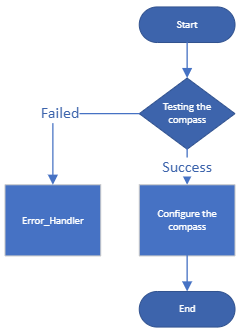
\includegraphics[scale=.6]{figures/6.png}
        \caption{Flow Chart of initiating function}
    \end{figure}
    \begin{itemize}
        \item This function takes the I2C peripheral used to communicate with the module as input.
        \item The function does not return.
        \item It starts by testing the compass using the function \textbf{HAL\_Compass\_Test}.
        \item if the test is successful, the code continues. If the test is failed, the function \textbf{Error\_Handler} is called. This function is configurable by the user.
        \item The configuration set by the user as discussed earlier would be set for the module.
    \end{itemize}
    
    
    \item \textbf{void HAL\_Compass\_Get(I2C\_HandleTypeDef *I2Cx, Compass\_TypeDef *DataStruct)}
    \begin{figure}[h]
        \centering
        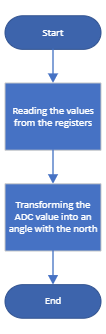
\includegraphics[scale=.8]{figures/7.png}
        \caption{Flow Chart of getting function}
    \end{figure}
    \begin{itemize}
        \item This function takes the I2C peripheral that communicate with module and a pointer to the data struct used to store the values of the angles as inputs.
        \item The function does not return.
        \item It starts by reading the values stored in the data registers of the sensor.
        \item It transforms these raw valued from the registers into an angle representing the angle between the axis and the north.
    \end{itemize}
    
    \clearpage
    \item \textbf{HAL\_StatusTypeDef HAL\_Compass\_Test(I2C\_HandleTypeDef *I2Cx)}
    \begin{figure}[h]
        \centering
        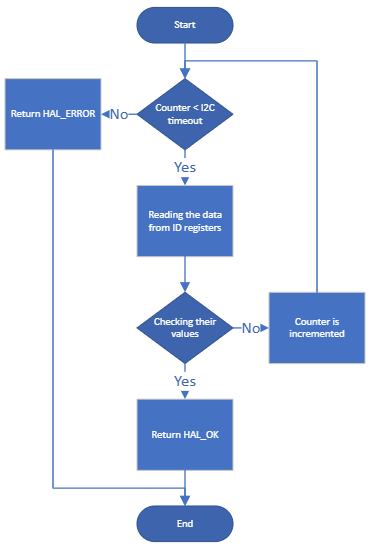
\includegraphics[scale=.6]{figures/8.png}
        \caption{Flow Chart of testing function}
    \end{figure}
    \begin{itemize}
        \item This function takes the I2C peripheral that communicates with the sensor as input.
        \item This function returns the status of the test.
        \item There are identification registers in the sensor, they are read only memory with fixed values.
        \item The function checks first the time out of the counter to see if the number of tries exceeded the allowed  number of iterations.
        \item Reading the value of the identification registers and comparing them with the default value of them.
        \item Returning HAL\_OK if the values are the same as the default values.
        \item Returning HAL\_ERROR if the values are not the same as the default and the number of tries exceeded the allowed number of iterations.
    \end{itemize}
\end{enumerate}
\subsection{Testing the sensor}
To test the sensor, its output is compared with values from external compass like the compass in most phones.
Theoretically, the two values should be the same.
When testing this sensor, the values from the sensor have offset by a value ranging from 1 degree to 7 degrees from the external compass.

\section{Location Measurement Unit}
Now, location for the vehicle needs to be measured, there were two options:
\begin{enumerate}
    \item GPS Data: It can be extracted from a GPS module, but as said before, the available modules need a very clear light of side to communicate with a satellite, so it was replaced with a Bluetooth module connecting with a mobile phone to get the GPS data from it since the mobile has a very accurate internal GPS.
    \newline The needed data from GPS was the longitude and latitude to determine exactly the vehicle position.
    \item Ultra sonic mechanism: Although GPS from mobile is more accurate than any single GPS module, it is has an error that may be affected on the calculations and analysis. Ultra sonic mechanism is very easy way to determine the distance between two device, it sends a chirp from the source, when it meets a surface, an echo reflected to the source. From the speed of echo and time it calculates the distance. This method is more accurate than GPS data.
\end{enumerate}

Despite of Ultra sonic accuracy, GPS data are extracted and used, it will help in some applications that will be discussed in chapter 9.

\subsection{Data collection from the module}
\begin{wrapfigure}{r}{5cm}
    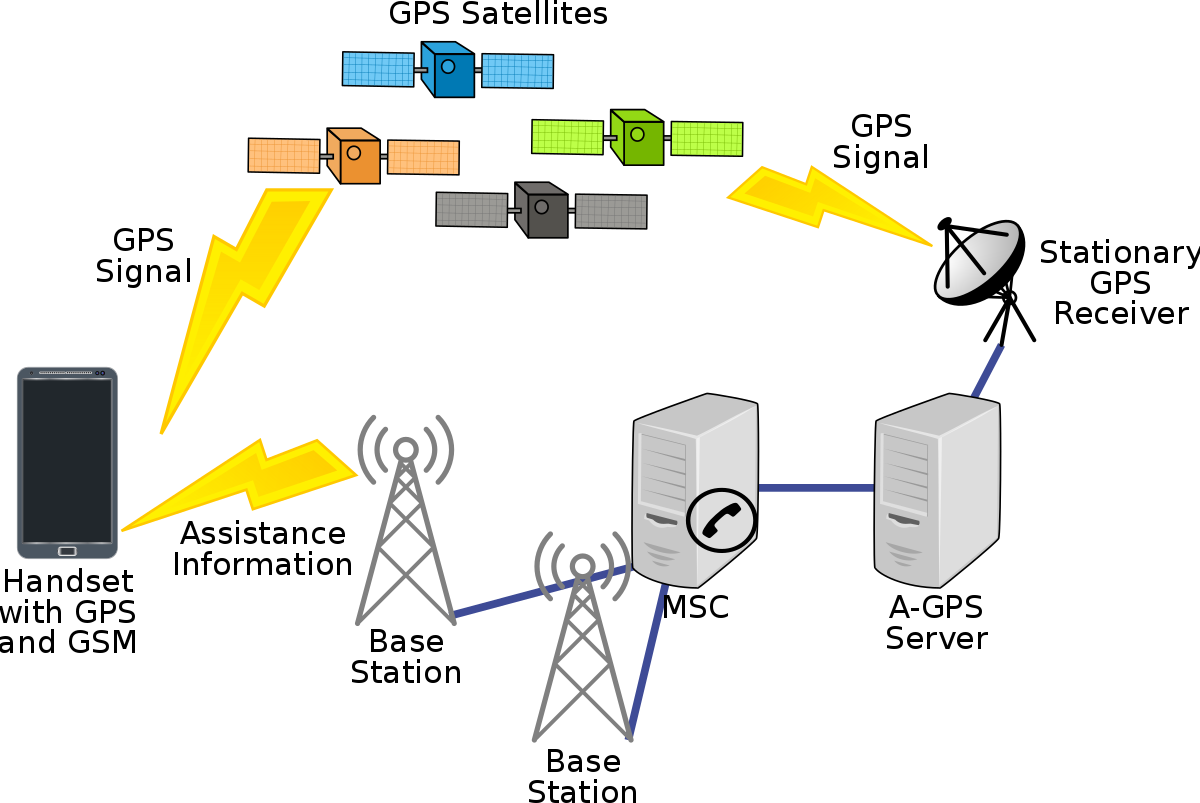
\includegraphics[width=0.5\textwidth]{figure/5_7.png}
    \caption{GPS block diagram in communication system}
    \label{fig:gps-block}
\end{wrapfigure}
The GPS module contains tiny processors and antennas that receive data sent from
the satellite through dedicated RF frequencies. From there, it’ll receive timestamps
from each visible satellite, along with other pieces of data. If the module’s antenna
can spot 4 or more satellites, it’s ability to accurately calculate its position and time,
which means this is the circuit that will allow us to know each car’s position
accurately.

\subsubsection{GPS Features}
\begin{itemize}
    \item Cold start time of 38 s and Hot start time of 1s.
    \item Supply voltage: 3.3 V.
    \item Configurable from 4800 Baud to 115200 Baud rates. (default 9600).
    \item SuperSense ® Indoor GPS: -162 dBm tracking sensitivity.
    \item 5Hz position update rate.
    \item Operating temperature range: -40 TO 85°C.
    \item UART TTL socket.
    \item EEprom to save configuration settings.
    \item Rechargeable battery for Backup.
    \item Separated 18X18mm GPS antenna.

\end{itemize}


\subsubsection{GPS working principle}
As shown in figure \ref{fig:gps-block}, there are three major segments in GNSS/GPS system:
\begin{enumerate}
    \item Space Segment (satellites)
    \begin{itemize}
        \item 24-32 MEO satellites.
        \item Obital period of 11 hr 55 min.
        \item 20,200 km Altitude above Earth.
        \item 5 to 8 satellites visible at all times from any
location any where in the world.
        \item These satellites have VERY accurate clocks on
board.
        \item The satellites continuously send radio signals
towards earth.
        \item These radio signals are picked up by GPS
receivers.

    \end{itemize}
    
    \item Control Space
    \begin{itemize}
        \item Control stations enable information on Earth to be
      transmitted to the satellites (updates and fine turning).
      \item Control stations continuously track satellites, and update the
positions of each satellite.
      \item Without control stations, the accuracy of the system would degrade in a matter of days.
    \end{itemize}
    
    \item User Segment (GNSS Receivers or units)
    \begin{itemize}
        \item GPS units are referred to as “receivers”.
         \item They receive information (radio signals) from satellites.
         \item They calculate current position and speed/direction
    \end{itemize}
\end{enumerate}

The user segment receives RF signal from GPS at time 't'. Using this time with the speed of light, distance is calculated (R = C * t).
\newline
R value now represents just one plane but the earth is a sphere (3D), so it is needed to calculate R values for three planes to calculate the location point for the receiver.
\newline Thus the receiver has to communicate with three satellite with three equation as shown in figure \ref{fig:gps-equations}.

    \begin{figure}[h]
    \centering
    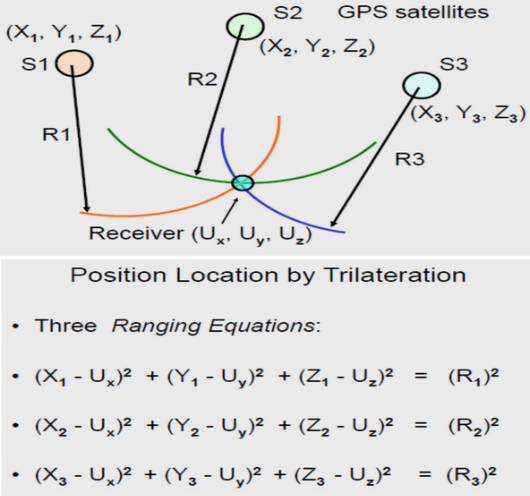
\includegraphics[width = .8\textwidth]{figure/5_8.png}
    \caption{GPS equations}
    \label{fig:gps-equations}
    \end{figure}
    
$X_i$, $Y_i$, and $Z_i$ refer for ith satellite position. \\
$U_x$, $U_y$ and $U_z$ are unknown and they are calculated by solving the three equation, they indicate the receiver position.
 
\subsubsection{GPS Timing}

\begin{itemize}
    \item Each GPS Satellite carries four highly accurate atomic clocks which provide GPS time.
    \item Civil receivers do not have atomic clocks (moderately
     accurate quartz clocks).
     \item Receiver clock must be synchronized to GPS time.
     \item  Requires 4th satellite (fourth equation) to solve for clock bias/error.
     \item Four unknowns are $U_x$, $U_y$, $U_z$, and T.
\end{itemize}

Now, four satellites with four equations are needed to solve timing problem as shown in figure \ref{fig:gps-equationss-time}.

    \begin{figure}[h]
    \centering
    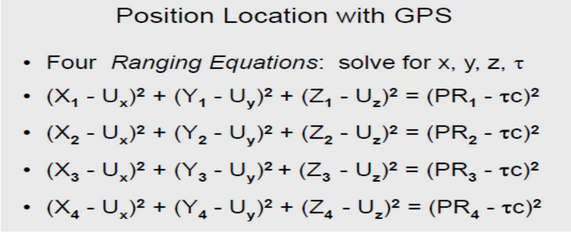
\includegraphics[width = \textwidth]{figure/5_9.png}
    \caption{GPS equations for timing solving}
    \label{fig:gps-equationss-time}
    \end{figure}
 \newpage   
\subsubsection{Receiving GPS data using Bluetooth module}

Bluetooth module communicates with the mobile phone using an Android application called "Share GPS" to get the data as shown in figures \ref{fig:mobile-bt1} and \ref{fig:mobile-bt2}. After successful connection, Bluetooth module shares this data with STM using UART, in next sections configurations and used functions will be discussed.\newpage

\begin{figure}[h]
    \centering
    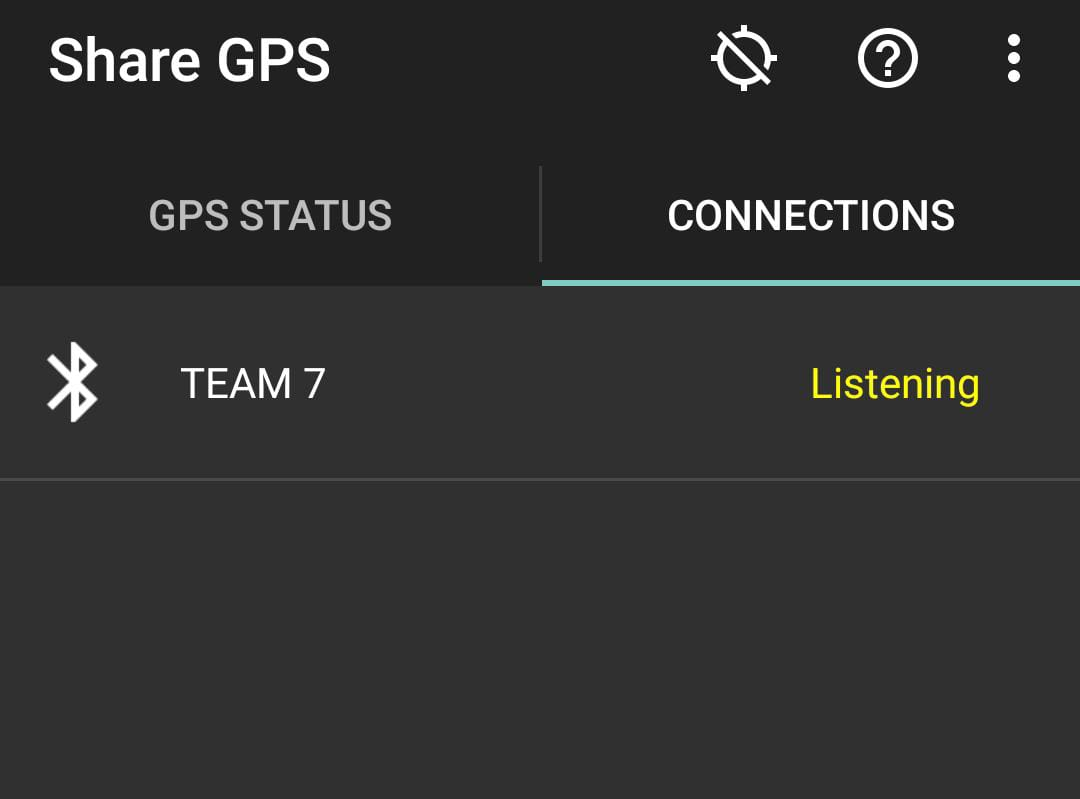
\includegraphics[width = .8\textwidth]{figure/5_10.jpg}
    \caption{Mobile phone is listening to Bluetooth module}
    \label{fig:mobile-bt1}
    \end{figure}
    
\begin{figure}[h]
    \centering
    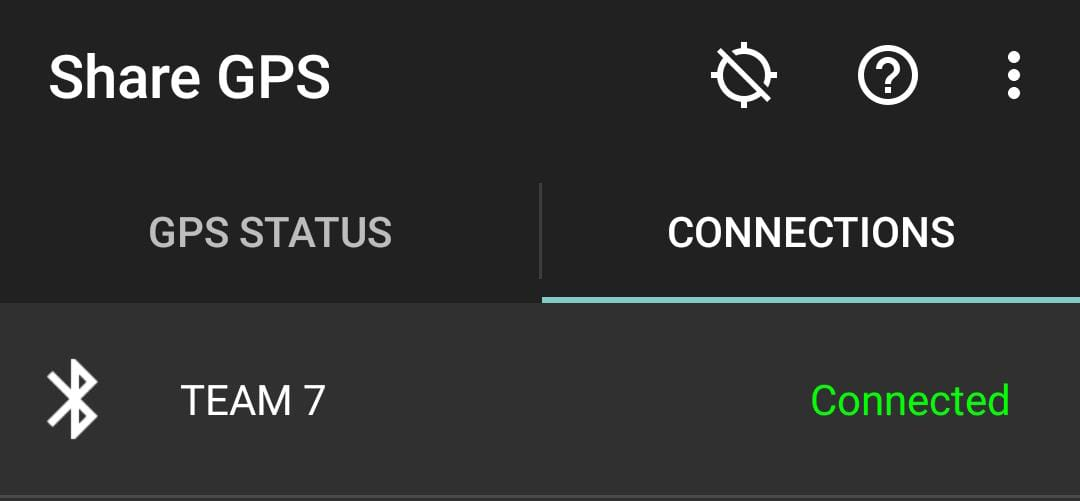
\includegraphics[width = .8\textwidth]{figure/5_11.jpg}
    \caption{Mobile phone connected to Bluetooth module}
    \label{fig:mobile-bt2}
    \end{figure}
  \newpage  
% \subsubsection{2. Ultra Sonic}
% Ultrasonic used to determine whether or not there is an obstacle ahead and measure
% the distance in small ranges smaller than 1M. \\
% The module used in project is HC-RS04 that connection consist of trig and echo pins ash shown in the figure.

% \begin{figure}[h]
%     \centering
%     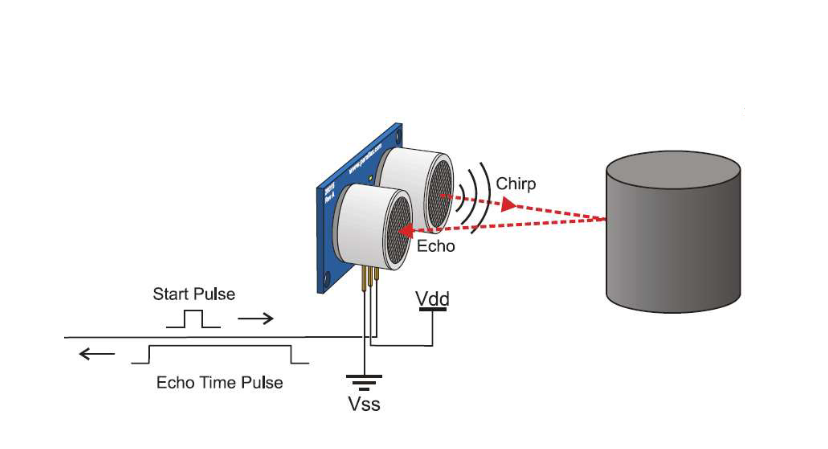
\includegraphics[width = \textwidth]{figure/5_12.PNG}
%     \caption{Ultra sonic diagram}
% \end{figure}

\subsection{Configuration Tools}

Bluetooth module needs UART configuration to communicate with the STM, USART3 is configured with NVIC enable as shown in figure \ref{fig:uart-config-bt}.

\begin{figure}[h]
    \centering
    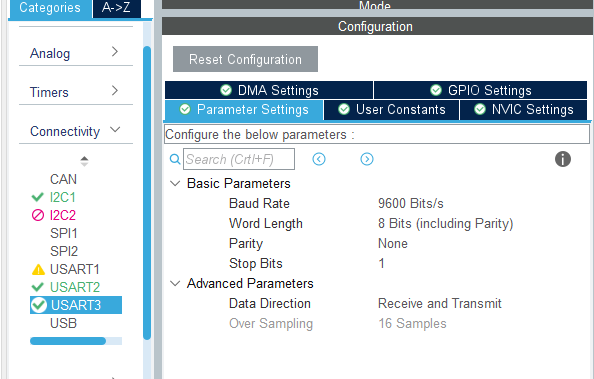
\includegraphics[width = .8\textwidth]{figure/5_13.PNG}
    \caption{UART configuration for Bluetooth module}
    \label{fig:uart-config-bt}
    \end{figure}
 
Enabling NVIC allows usage of UARTRingBuffer library; it is a library that helps in transmitting and receiving data from/to STM By a ring (circular) buffer as shown in figure \ref{fig:uart-ring}  which will be compatible with GPS data since the size of buffer needed for this data isn't constant.

\begin{figure}[h]
    \centering
    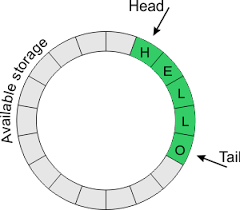
\includegraphics[width = .4\textwidth]{figure/5_14.png}
    \caption{UART ring buffer mechanism}
    \label{fig:uart-ring}
    \end{figure}
\newpage 

\subsection{Used functions}

In this section all implemented and used functions will be discussed. \\ First of all, USART3 and ringbuffer are initialized, then the algorithm for the code waits for "RMC" value from GPS, when it's received, the data after it until char '*' will be copied at buffer "RMC", finally \textbf{getGPSData()} is called to get the longitude, latitude, longitude direction, and latitude direction into GPS data structure.\\ RMC command and character '*' will be discussed in chapter 6.

\textbf{The code in main function:}

\begin{lstlisting}

int main()
{
    MX_USART3_UART_Init();
     Ringbuf_init();
    while(1)
    {
        if(Wait_for("RMC") == 1)
	  {
	  	Copy_upto("*", RMC);
	  	getGPSData();

	  }
    }
}

\end{lstlisting}

\subsubsection{getGPSData():}
Going deeply into this function, this function extracts both longitude and latitude neglecting any other received characters (i.e, neglecting ',' character between values), each one is extracted in temporary array to be converted into string using \textbf{atof()} function which is an internal function in C language in which converts array into float number. For directions, they are only one character for them, so they are easy to be extracted and stored in character variables. This implementation must be done when the data is received successfully and the data is valid, this check is done by an if condition in the beginning of the function.

\textbf{getGPSData() part for calculation latitude and latitude direction (this code is the same for longitude data replacing latitude variables with longitude ones):}

\begin{lstlisting}

void getGPSData(void)
{
	while(RMC[indexRMC] == ',') indexRMC++;
	while(RMC[indexRMC] != ',') indexRMC++;

	while(RMC[indexRMC] == ',') indexRMC++;
	gpsData.valid = RMC[indexRMC++];

	if(gpsData.valid == 'V' || gpsData.valid == 'N')
	{
		/* Get latitude */
		indexTempArray = 0;
		tempArray[indexTempArray++] = '0';
		tempArray[indexTempArray++] = '.';
		while(RMC[indexRMC] == ',') indexRMC++;
		while(RMC[indexRMC] != ',')
		{
			if(count == 0)
			{
				if(RMC[indexRMC] == '0') count--;
				gpsData.latitude = (RMC[indexRMC] - '0') * 10;
			}
			else if(count == 1)
			{
				gpsData.latitude += (RMC[indexRMC] - '0');
			}
			else
			{
				if(RMC[indexRMC] != '.')
					tempArray[indexTempArray] = RMC[indexRMC];
				indexTempArray++;

			}
			count++;
			indexRMC++;
		}
		gpsData.latitude += (atof(tempArray) / 60);
		for(globalIndex = 0; globalIndex < 20; globalIndex++)
			tempArray[globalIndex] = '0';
		count = 0;


		/* Get latitude direction */
		while(RMC[indexRMC] == ',') indexRMC++;
		gpsData.dirLatitude = RMC[indexRMC++];


\end{lstlisting}

\subsection{Testing}

The test is done by debugging this variables using STMCube IDE debugger which helps to trace the code line by line.

GPS data structure:
\begin{lstlisting}
typedef struct DataGPS
{
	float longitude;
	float latitude;
	char dirLongitude;
	char dirLatitude;
	char valid;
}gps_t;

\end{lstlisting}

This structure is traced and viewed. To ensure that they are correct values, they are compared with GPS data in the mobile phone, if they are similar then the code works properly. \\

There is a bug in waitfor() function; if it didn't receive RMC, the code will stop in this line infinitely causing error fault. This is done when the power is on, so the STM must be reset when this bug happens.

\section{Sharing-With-Server Unit}
In this section, the discussion will be about how Raspberry Pi and STM exchange data together. Raspberry Pi is chosen due to some features that whill be discussed in next sub-section.

\subsection{Data Collection}

STM and Raspberry Pi communicate with UART protocol to send and receive data that is being shared with the server. Raspberry pi is an efficient IC that has a very strong processor. Although Raspberrpy Pi is expensive compared to other ICs, this is chosen in the project because it will be a suitable component for the applications that will be integrated in the project. Raspberry pi supports GUI, so it will be a good choice for implementing it with the display for showing the data for the user.

\subsubsection{Raspberry Pi features}
\begin{itemize}
    \item 512 MB SDRAM memory.
    \item Broadcom BCM2835 SoC full high definition  multimedia processor.
    \item Dual Core Video Core IV Multimedia coprocessor.
    \item Single 2.0 USB connector.
    \item HDMI (rev 1.3 and 1.4) Composite RCA (PAL & NTSC) Video Out.
    \item 3.5 MM Jack, HDMI Audio Out.
    \item MMC, SD, SDIO Card slot on board storage.
    \item Linux Operating system.
    \item Linux Operating system.
    \item  On board 10/100 Ethernet RJ45 jack.
\end{itemize}
    
\subsubsection{Connecting raspberry with PC}
Raspberry Pi has a linux terminal that can be accessed using a software called "PuTTy" as shown in figure  \ref{fig:putty-config}. By connecting the raspberry with the PC using an Ethernet cable and a USB cable as shown in figure \ref{fig:ether-rasp}, the terminal will be ready on the software and the Raspberry Pi has been successfully accessed. \\

\begin{figure}[h]
    \centering
    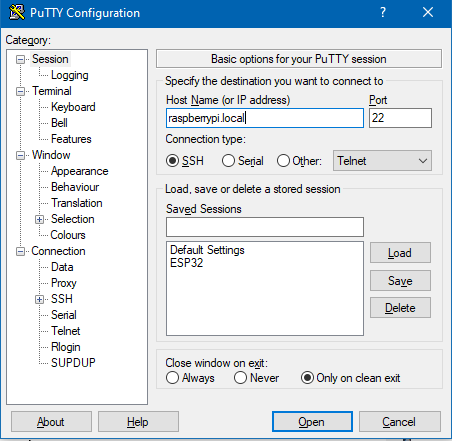
\includegraphics[width = .75\textwidth]{figure/5_15.PNG}
    \caption{PuTTy configuration to connect Raspberry Pi with PC}
    \label{fig:putty-config}
    \end{figure}
\newpage 

\begin{figure}[h]
    \centering
    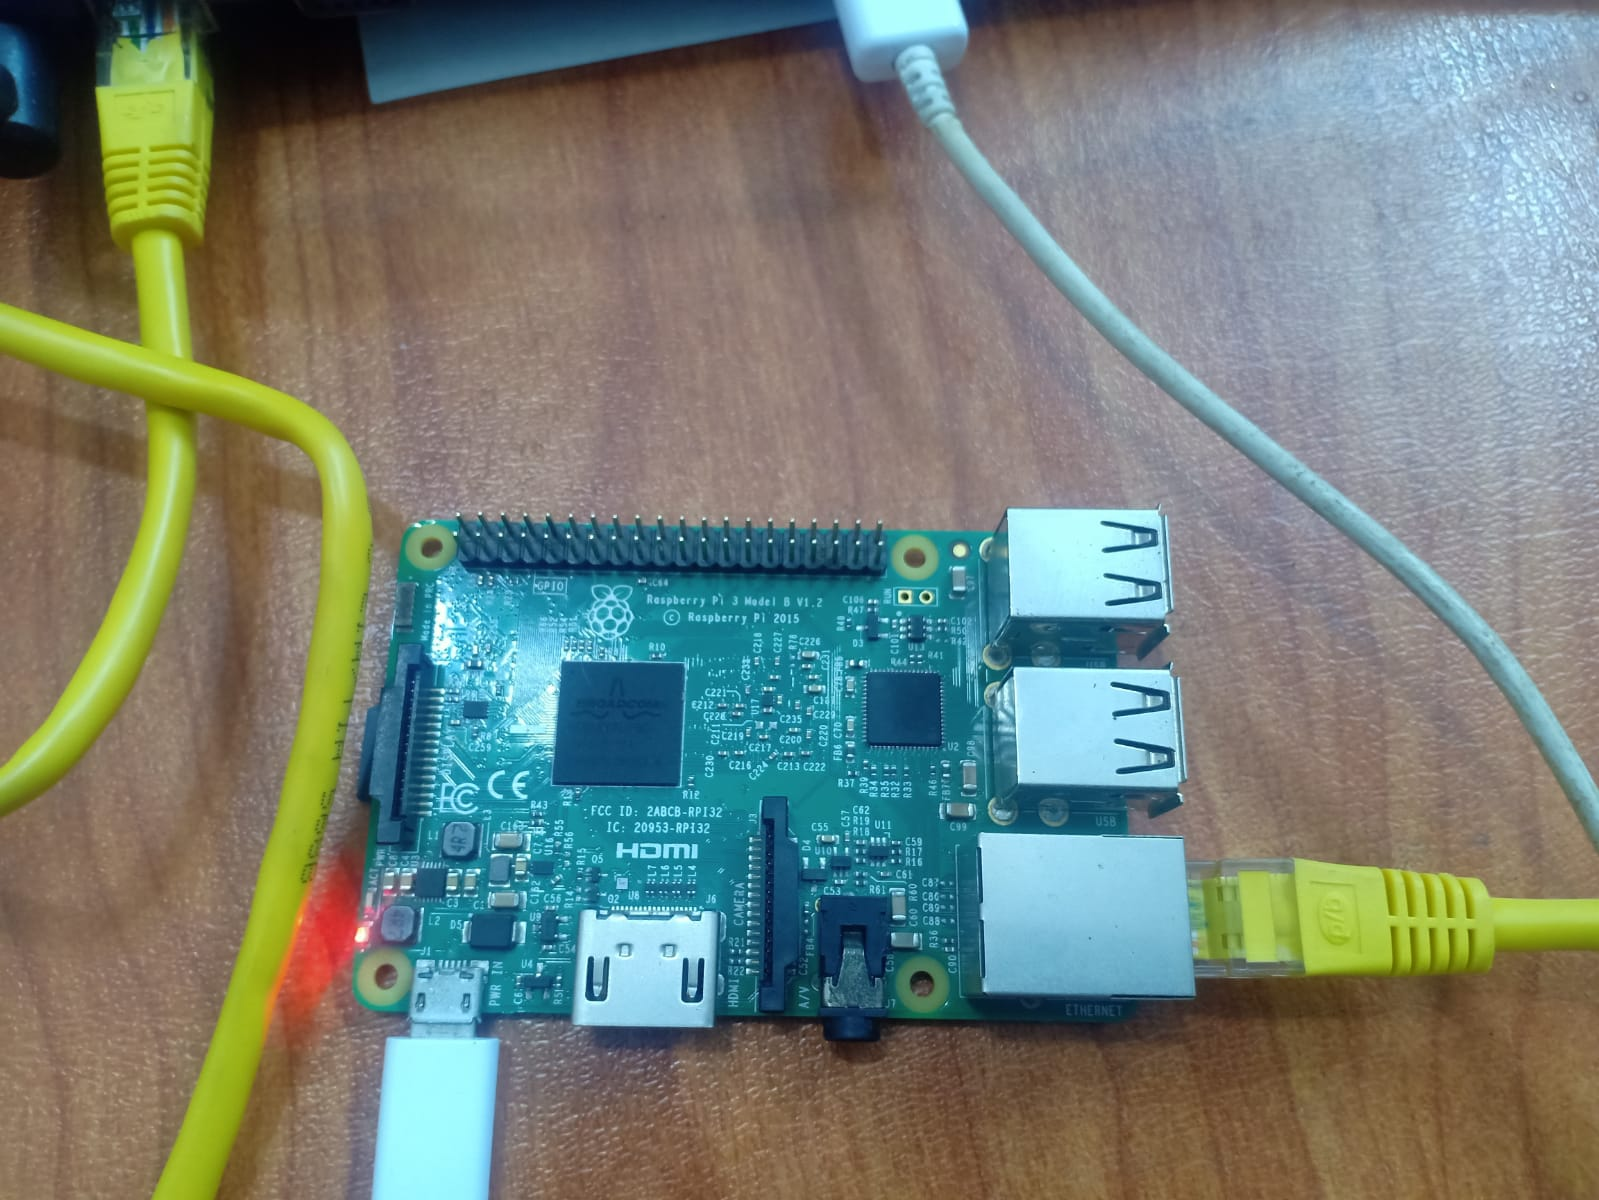
\includegraphics[width = .7\textwidth]{figure/5_16.jpg}
    \caption{Raspberry Pi hardware connection with PC}
    \label{fig:ether-rasp}
    \end{figure}
\clearpage 
\subsubsection{Notes}
\begin{enumerate}
    \item You can access the Raspberry Pi with HDMI screens that will provide you with a full GUI that will be easier to deal with than the Linux terminal.
    \item If the raspberry is too expensive to buy, you can replace it with any IC that provides a Wi-Fi protocol (i.e, ESP32 is suitable).
    \item If there is a problem with opening the terminal in PuTTy, try to allow sharing in adapter options from windows network settings.
\end{enumerate}

Going back to PuTTy, after wiring "raspberrypi.local" in host name then  pressing on "connect", the terminal of Raspberry will be opened and it will be required to enter your user name and password as shown in figure \ref{fig:rasp-terminal}, the default for all raspberries are:
\begin{enumerate}
    \item user name -  pi
    \item password  -  raspberry
\end{enumerate}

    
\begin{figure}[h]
    \centering
    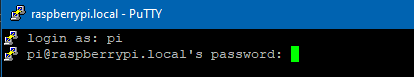
\includegraphics[width = \textwidth]{figure/5_17.PNG}
    \caption{Raspberry Pi terminal for user name and password}
    \label{fig:rasp-terminal}
    \end{figure}
\newpage 

After writing the user name and the password, the operating system opened as shown in figure \ref{fig:rasp-os}, you are now on the home in the raspberry Linux, if you wrote "nano UART.py"command, it will generate this file with python extension. \\
To run UART.py, use "python UART.py" command.
So, python file is written for enable UART for raspberry using serial library. In next sub-section the used python code will be showed.

\begin{figure}[h]
    \centering
    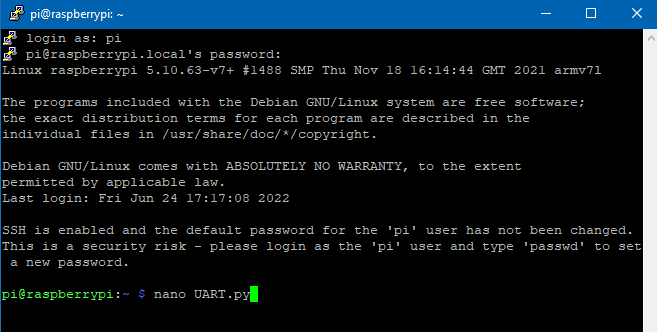
\includegraphics[width = \textwidth]{figure/5_18.PNG}
    \caption{Raspberry Pi operating system terminal}
    \label{fig:rasp-os}
    \end{figure}
\newpage 
    
In next sections, the configuration of STM and used functions in both Raspberry Pi will be discussed.

\subsection{Configuration Tools}

In STMCube, USART2 is enabled as shown in figure \ref{fig:uart-config-rasp}, note that the baud rate changed to 115200 since the raspberry baud rate is 115200, so the two devices must have the same baud rate.

\begin{figure}[h]
    \centering
    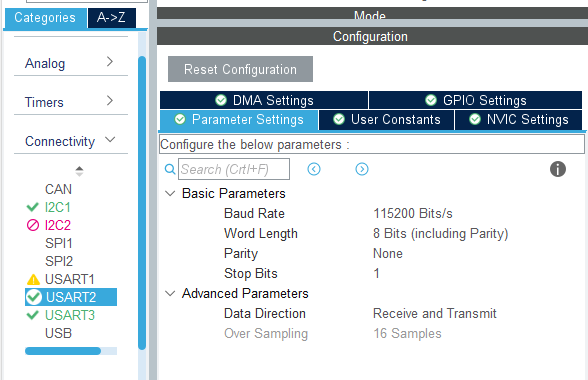
\includegraphics[width = \textwidth]{figure/5_19.PNG}
    \caption{UART configuration  in STM for connection with Raspberry Pi}
    \label{fig:uart-config-rasp}
\end{figure}

As will be seen in next sub-section, the functions are in blocking mode, so no need to enable NVIC.

\subsection{Functions Used}
In this section functions used in both raspberry and STM are discussed.

\subsubsection{1. STM}

In the main function the code sequence is written as follow:

\begin{enumerate}
    \item Initialization of UART2 before while loop.\\
    \textbf{Then inside while loop:}
    \item Automatic generated function \textbf{HAL\textunderscore UART\textunderscore Receive()} is called to receive data from the raspberry and store it into a buffer called BufferRX.
    \item \textbf{resetBuffersIndexes()} function is called to reset all indexes before entering in implementation to avoid any garbage error.
    \item \textbf{getNeighborData()} function is called to extract the data received into their suitable variables in neighbor data structure.
    \item \textbf{getCarData()} function is called to extract the data from the sensors into their suitable variables in car data structure.
    \item \textbf{analysis() }function is called to analysis this data, this is will be discussed in details in chapter 6.
    \item \textbf{generateTransmitBuffer()} function in called to insert the values in car data structure into a buffer called be BufferTX.
    \item  Automatic generated function \textbf{HAL\textunderscore UART \textunderscore Transmit()} is called to transmit data stored in BufferTX from the STM to Raspberry Pi.
\end{enumerate}

Going deeply into each manually written functions:

\subsubsection{A. main()}
\begin{lstlisting}
int main()
{
    MX_USART2_UART_Init();
    while(1)
    {
      HAL_UART_Receive(&huart2, bufferRX, sizeof(bufferRX), 0xFFFF);
	  resetBuffersIndexes();
	  getNeighborData();
	  getCarData();
	  analysis();
	  generateTransmitBuffer();
	  HAL_UART_Transmit(&huart2, bufferTX, sizeof(bufferTX), 0xFF);
    }
}
\end{lstlisting}

\subsubsection{B. resetBuffersIndexes()}
\begin{lstlisting}
void resetBuffersIndexes(void)
{
	indexBufferTX = 0;
	indexBufferRX = 0;
}

\end{lstlisting}

\subsubsection{C. getNeighborData()}
\begin{lstlisting}
void getNeighborData(void)
{
	// Get longitude
	neighbor.longitude = splitData();

	// Get latitude
	indexBufferRX++;
	neighbor.latitude = splitData();

	// Get speed
	indexBufferRX++;
	neighbor.speed = splitData();

	// Get Ax
	indexBufferRX++;
	neighbor.Ax = splitData();

	// Get Ay
	indexBufferRX++;
	neighbor.Ay = splitData();

	// Get Angle
	indexBufferRX++;
	neighbor.angle = splitData();

	// Get Vx
	indexBufferRX++;
	neighbor.Vx = splitData();

	// Get Vy
	indexBufferRX++;
	neighbor.Vy = splitData();
}
\end{lstlisting}

\subsubsection{D. getCarData()}
\begin{lstlisting}
void getCarData(void)
{
	car.longitude = gpsData.longitude;
	car.latitude  = gpsData.latitude;
	car.speed     = (float) hrotary.RPM;
	car.Ax        = (float) himu.Ax;
	car.Ay        = (float) himu.Ay;
	car.angle     = 30.001001;
	car.Vx        = car.speed * (sin((car.angle *PI)/180));
	car.Vy        = car.speed * (cos((car.angle *PI)/180));
}
\end{lstlisting}

\subsubsection{E. generateTransmitBuffer()}
\begin{lstlisting}
void generateTransmitBuffer(void)
{
	bufferTX[indexBufferTX++] = 'D';
	bufferTX[indexBufferTX++] = ':';

	mergeData(car.longitude);
	mergeData(car.latitude);
	mergeData(car.speed);
	mergeData(car.Ax);
	mergeData(car.Ay);
	mergeData(car.angle);
	mergeData(car.Vx);
	mergeData(car.Vy);
	bufferTX[indexBufferTX++] = '?';

	for(; indexBufferTX < TX_SIZE; indexBufferTX++)
	{
		bufferTX[indexBufferTX] = '!';
	}
}
\end{lstlisting}

\textbf{splitData()} is used to help in splitting the BufferRx into a separate variables. i.e, BufferRX contains values of speed, acceleration, longitude, latitude,..etc, the function splits these values into their specific variables.

\textbf{mergeData()} is used to help in merging the separate values into BufferTX. i.e, specific variables that represent values of speed, acceleration, longitude, latitude,..etc, the function merges these values into BufferTX.

\subsubsection{splitData()}
\begin{lstlisting}
float splitData(void)
{
	indexTempArray = 0;
	while(bufferRX[indexBufferRX] != ',' && bufferRX[indexBufferRX] != '!')
	{
		tempArray[indexTempArray] = bufferRX[indexBufferRX];
		if(bufferRX[indexBufferRX] == '.') checkInt = 0;
		indexTempArray++;
		indexBufferRX++;
	}
	if(checkInt == 1) tempArray[indexTempArray] = '.';
	checkInt = 1;
	splitValue = atof(tempArray);
	for(globalIndex = 0; globalIndex < 20; globalIndex++)
		tempArray[globalIndex] = '0';
	return splitValue;
}
\end{lstlisting}

\subsubsection{mergeData()}
\begin{lstlisting}
void mergeData(float value)
{

	gcvt(value, TEMP_ARR_SIZE, tempArray);

	for(indexTempArray = 0; indexTempArray < MAX_FLOAT_DIGITS; indexTempArray++)
	{
		if(tempArray[indexTempArray] == '\0') break;
		bufferTX[indexBufferTX] = tempArray[indexTempArray];
		indexBufferTX++;
	}
	bufferTX[indexBufferTX++] = ',';


	for(globalIndex = 0; globalIndex < TEMP_ARR_SIZE; globalIndex++)
		tempArray[globalIndex] = '0';
}

\end{lstlisting}

\subsubsection{2. Raspberry Pi}

In the UART function the code sequence is written as follow:

\begin{enumerate}
    \item Serial library and server libraries are imported.
    \item Size of buffers is initialized.
    \item Message is extracted from JSON file into a string variable, this will be discussed in details in chapter 7.
    \item Adding redundant characters to complete the size of the buffer. \\ \textbf{}{Inside while true loop:}
    \item Data is sent to STM using \textbf{ser.write()}
    \item Data is received from STM using \textbf{ser.read()}
    \item Try catch statement is inserted to avoid any errors in encoding and decoding.
\end{enumerate}

\subsubsection{UART() code: }



\begin{lstlisting}
ser = serial.Serial()
ser.port = '/dev/ttyAMA0'
ser.baudrate = 115200
ser.timeout = 60
ser.open()

TXSize = 50
RXSize = 50
msgReceived = ''

#msgSent = input("Write: ")
msgSent = read_file("test.json")
msgSent = format_json_string(msgSent)
for i in range(len(msgSent), TXSize):
    msgSent += '.'
ser.write(msgSent.encode())
while True:
    msgReceived = ser.read(RXSize)
    try:
        msgReceived.decode()
        print(msgReceived)
        write_json_file("received-test.json", msgReceived)
    except (UnicodeDecodeError, AttributeError):
        print("error")
        pass
    if msgReceived == b'\r':

        break
\end{lstlisting}

UART function is inserted into the main python file that is responsible for running all written code in raspberry, that will be discussed in chapter 8.

\subsection{Testing}
For STM, the testing is done by tracing the code line by line using the debugger in STMCube IDE, it helps for studying the values of each structure continuously, so errors are found out easier. 
For raspberry Pi, printing the message received helps for ensuring that the data received successfully. 

\subsubsection{1. Car Data structure in STM}
\begin{lstlisting}
typedef struct CarData
{
	float longitude;
	float latitude;
	float speed;
	float Ax;
	float Ay;
	float angle;
	float Vx;
	float Vy;
	float dx;
	float dy;
	float x2;
	float y2;
}data_t;
\end{lstlisting}

\subsubsection{2. Printed message on Raspberry Pi}
The message received on STM is displayed as shown in figure \ref{fig:output-rasp}, to ensure that the reception is successful, it is compared with BufferTx in STM and they must be the same. The label for the message is discussed in chapter 6.

\begin{figure}[h]
    \centering
    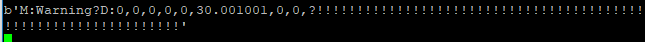
\includegraphics[width = \textwidth]{figure/5_20.PNG}
    \caption{Output message in Raspberry}
    \label{fig:output-rasp}
    \end{figure}
\newpage 

\subsubsection{Testing Steps}
\begin{enumerate}
    \item UART is tested by only one character.
    \item Test using a manual data.
    \item Test using sensor data.
    \item Test using JSON files.
    \item Test with the server.
\end{enumerate}